\chapter{Algebrización de Variedades Complejas}

	Hasta este punto hemos introducido diversas herramientas cuya motivación está dada por la pregunta: ¿cuándo puede una variedad compleja describirse mediante ecuaciones algebraicas?
	
	\begin{definition}
		Una variedad compleja se dice \textbf{algebrizable}, o se dice que \textbf{admite una estructura algebraica}, si es biholomorfa a una variedad algebraica $V\subset \pp^N$.
	\end{definition}
	
	Si $M$ es una variedad compleja algebrizable, a la variedad algebraica $V\subset \pp^N$ se le denomina \textbf{realización} de $M$\footnote{También se suele decir que $M$ se \textbf{realiza} como la variedad algebraica $V$.}. Por el Teorema \ref{varalg}, toda variedad algebraica es conexa y compacta; y en consecuencia, en todo este trabajo nos hemos enfocado principalmente en variedades complejas con estas propiedades topológicas, pues toda variedad compleja algebrizable necesariamente debe ser conexa y compacta.
	
	En este último capítulo retomaremos todas las herramientas introducidas anteriormente para darle sentido a la pregunta de algebrización y exponer los criterios que nos permiten determinar cuándo una variedad compleja admite una estructura algebraica.

    \section{Subvariedades Analíticas}
    
    Antes de estudiar la algebrización de variedades, debemos introducir los últimos objetos fundamentales del trabajo.
    
    \begin{definition}[Subconjunto analítico]
    	Sea $M$ una variedad compleja. Un \textbf{subconjunto analítico} de $M$ es un subconjunto cerrado $V\subset M$ con la siguiente propiedad: para cada punto $x\in V$ existe una vecindad $U\subset M$ de $x$ tal que
    	\begin{equation*}
    		U\cap V=\{z\in U:f_1(z)=\cdots=f_k(z)=0\}
    	\end{equation*}  
    	para algunas funciones holomorfas $f_1,\dots,f_k\in\oo_M(U)$.
    \end{definition}
    
    Todo conjuntos algebraico de $\cc$ o $\pp^n$ son subconjuntos analíticos. Así, los subconjuntos analíticos son una generalización de los conjuntos algebraicos para otras variedades complejas.
    
    \begin{definition}[No singular]
    	Sea $M$ una variedad compleja y $V$ un subconjunto analítico de $M$. Decimos que $x\in V$ es \textbf{regular} o \textbf{no singular} si existe una carta $(U,\varphi)$ de $M$ alrededor de $x$ tal que $U\cap V=Z(f_1,\dots,f_k)$ y $\varphi(x)\in \varphi(U)$ es un punto regular de la aplicación
    	\begin{equation*}
    		f:=(f_1\circ\varphi^{-1},\dots,f_k\circ\varphi^{-1}):\varphi(U)\longrightarrow \cc^k.
    	\end{equation*}
    	Es decir, la jacobiana de $f$ en $\varphi(x)$ tiene rango $k$. Denotamos por $V^*$ al conjunto de todos los puntos regulares de $V$.
    	
    	Los puntos del conjunto $V_s:=V\setminus V^*$ son llamados \textbf{puntos singulares}. Por último, decimos que $V$ es \textbf{no singular} si $V_s=\emptyset$, es decir, si $V$ es una subvariedad compleja de $M$ (véase observación \ref{subvariedadesporecuaciones}).
    \end{definition}
    
    Los subconjuntos analíticos pueden interpretarse como variedades complejas que permiten singularidades. Aunque estas singularidades serán solo un subconjunto cerrado y al igual que las variedades algebraicas, los puntos regulares formarán un subconjunto denso. Esto implica que las subvariedades analíticas se comportan como subvariedades complejas con una muy pequeña cantidad de singularidades.
    
    \begin{propo}\parencite[Chap 0, Sec. 2.2]{griffiths}\label{puntossingulares}
    	Sea $M$ una variedad compleja y $V\subset M$ un subconjunto analítico. Entonces el conjuntos de puntos singulares $V_s$ está contenido en un subconjunto analítico de $M$ no igual a $V$.
    \end{propo} 
%    \begin{proof}
%    	Tomemos $p\in V$ y una vecindad $U$ de $p$ tal que
%    	\begin{equation*}
%    		V\cap U=Z(f_1,\dots, f_r),\qquad f_i\in\oo_M(U).
%    	\end{equation*}
%    	Sea $J(f)$ la matriz jacobiana de la aplicación $f=(f_1,\dots,f_r)$. Definamos
%    	\begin{equation*}
%    		k=\max_{q\in V\cap U}\operatorname{rk} J(f)(q).
%    	\end{equation*}
%    	Entonces el conjunto
%    	\begin{equation*}
%    		W=\{q\in V\cap U:\mathrm{rk}J(f)(q)<k\}
%    	\end{equation*}
%    	está definido por la anulación de todos los menores $k\times k$, por lo que es un subconjunto analítico de $V\cap U$. En particular, $W\neq V\cap U$ pues existe al menos una menor $k\times k$ que no se anula idénticamente en $V\cap U$. De esta manera,
%    	\begin{equation*}
%    		V_s\cap U\subset W.
%    	\end{equation*}
%    	Por lo tanto, $V_s$ está contenido en un subconjunto analítico no igual a $V$.
%    \end{proof}
    
%    \begin{remark}
%    	Sea $V$ un subconjunto analítico de $M$ y $p\in V$ un punto no singular. Por definición, existe una vecindad $U$ de $p$ tal que
%    	\begin{equation*}
%    		V\cap U=Z(f_1,\cdots,f_k)
%    	\end{equation*}
%    	donde la función inducida en una carta tiene rango $k$. En particular, $p$ es un punto regular de $f$ y $f^{-1}(p)=V\cap U$ es una variedad compleja de dimensión $k$ (falta cita). Así, definimos 
%    	\begin{eqnarray*}
%    		\dim_p V:= k.
%    	\end{eqnarray*}
%    \end{remark}
   
    \begin{example}
    	Consideremos $D\subset \cc^n$ un conjunto discreto y cerrado no vacío. Esto significa que para todo punto $p=(p_1,\dots,p_n)\in D$ existe una vecindad del punto $U\subset\cc^n$ tal que
    	\begin{equation*}
    		U\cap D =\{p\}.
    	\end{equation*} 
    	Notemos que $Z(z_1-p_1,\cdots,z_n-p_n)=\{p\}$. Por lo tanto, $D$ es un subconjunto analítico de $\cc^n$.
    \end{example}
    
    \begin{remark}
    	Sabemos que los conjuntos algebraicos de $\mathbb{A}^1_\cc$ solo son conjuntos finitos. Por el ejemplo anterior, cualquier conjunto discreto $D$ en $\cc$ es analítico. Por lo tanto, los conjuntos algebraicos de  $\mathbb{A}^1_\cc$ también son analíticos, pero además, existen subconjuntos analíticos que no son algebraicos (véase ejemplo \ref{graficadelseno}).
    \end{remark}
    
    \begin{lemma}\label{preimagen analitico}
    	Sea $f:N\to M$ una aplicación holomorfa y $V\subset M$ un subconjunto analítico. Entonces $f^{-1}(V)\subset N$ es un subconjunto analítico.
    \end{lemma}
    \begin{proof}
    	Sea $V\subset M$ un subconjunto analítico y definamos $W=f^{-1}(V)$. Consideremos $p\in W$, entonces $f(p)\in V$. Como $V$ es analítico, existe una vecindad $U$ de $f(p)$ tal que
    	\begin{equation*}
    		U\cap V=Z(f_1,\dots,f_k)
    	\end{equation*} 
    	donde $f_1,\dots,f_k\in\oo_M(U)$. Luego, como $f$ es continua, $U'=f^{-1}(U)$ es una vecindad abierta de $p$. Definamos las funciones
    	\begin{equation*}
    		g_i=f_i\circ f:U'\to\cc,\quad i=1,2,\dots,k.
    	\end{equation*}
    	Notemos que las funciones $g_i$ son holomorfas, por ser composición de aplicaciones holomorfas. Así, 
    	\begin{align*}
    		U'\cap W&=f^{-1}(U\cap V)\\
    		&=f^{-1}(Z(f_1,\dots,f_k))\\
    		&=f^{-1}\left(\bigcap_{i=1}^k Z(f_i) \right)\\
    		&= \bigcap_{i=1}^k f^{-1}(Z(f_i))\\
    		&=\bigcap_{i=1}^k Z(f_i\circ f)\\
    		&=\bigcap_{i=1}^k Z(g_i)\\
    		&=Z(g_1,\dots,g_k).
    	\end{align*}
    	Por lo tanto, $W=f^{-1}(V)$ es un subconjunto analítico.
    \end{proof}
    
    \begin{definition}
    	Sea $M$ una variedad compleja y $V$ un subconjunto analítico de $M$. Decimos que $V$ es \textbf{irreducible} si no es posible escribirla como una unión $V=V_1\cup V_2$ de dos subconjuntos analíticos propios $V_i\subset V$ de $M$.\\
    	Un subconjunto analítico irreducible es llamado \textbf{subvariedad analítica}.
    \end{definition}
    
    \begin{corollary}
    	Sea $M$ una variedad compleja y $V$ un subconjunto analítico de $M$. Entonces el conjunto $V^*$ es denso en $V$ y una subvariedad compleja no vacía de $M$.
    \end{corollary}
    \begin{proof}
    	Supongamos que $V$ es irreducible. Sea $p\in V$ un punto regular, entonces existe una vecindad $U$ de $p$ tal que $V\cap U\subset V^*$ es una subvariedad compleja de $U$. De esta manera, $p$ es un punto interior de $V^*$. Con lo cual, $V^*$ es un abierto. 
    	
    	Por la proposición \ref{puntossingulares}, sabemos que existe un subconjunto analítico $W$ tal que
    	\begin{equation*}
    		V_s\subset W\subsetneqq V.
    	\end{equation*}
    	Como $W\neq V$, entonces $V^*=V\setminus V_s$ es no vacío. En particular, $V^*$ es una subvariedad compleja no vacía.
    	
    	Supongamos que $V_s$ contiene un abierto no vacío $A\subset V$. Entonces $A\subset W$. Dado que $V$ es irreducible y $W$ es un subconjunto analítico propio, por el teorema de la identidad, las funciones que definen a $W$ cerca de $A$ se deben anular siempre. Esto implica que $W=V$, lo cual es una contradicción. Con lo cual, $A$ es vacío.
    	
    	Si $V_s$ contuviera un abierto no vacío de $V$, entonces también lo contiene el subconjunto analítico $W$. Sin embargo, un subconjunto analítico propio de un subconjunto analítico irreducible no puede contener un abierto relativo. Por lo que, $V_s$ no contiene abiertos de $V$
    	
    	Como $V_s$ es cerrado en $V$ y no contiene abiertos de $V$, entonces
    	\begin{equation*}
    		\mathrm{Int}(V_s)=\emptyset.
    	\end{equation*}
    	Con lo cual, $V^*=V\setminus V_s$ es denso en $V$.
    	
    	Si $V$ no es irreducible, se aplica el argumento a cada componente irreducible $V_i$. Obteniendo que $V_i^*$ es denso en $V_i$, y por tanto la unión de todos los puntos regulares es densa en $V$.
    \end{proof}
    
    \begin{definition}
    	Sea $V\subset M$ una subvariedad analítica. Definimos la \textbf{dimensión} de $V\subset M$ como
    	\begin{equation*}
    		\dim V:=\dim V^*.
    	\end{equation*}
    	Es decir, la dimensión como subvariedad compleja de sus puntos no singulares.
    	
    	De igual manera, definimos la \textbf{codimensión} de $V$ como la codimensión de $V^*$.
    	Una \textbf{hipersuperficie analítica} es una subvariedad analítica de codimensión uno.
    \end{definition}
    
    \begin{remark}
    	Una consecuencia directa de la geometría local (véase proposición \ref{hipersuperficiesenCn}), es que toda hipersuperficie analítica en una variedad compleja $M$ está definida localmente como el conjunto de ceros de una sola función. Es decir, si $H\subset M$ es una hipersuperficie analítica, entonces para todo punto $p\in H$ existe una vecindad $U$ de $p$ y una función holomorfa $f\in \oo_M(U)$ irreducible tal que
    	\begin{equation*}
    		H\cap U=Z(f).
    	\end{equation*}
    \end{remark}
    
    \begin{example}
    	Consideremos la función holomorfa $y^2-x^2-x^3$ en $\cc^2$. Su conjunto de ceros es un subconjunto analítico en $\cc^2$, y de hecho es irreducible, por lo que
    	\begin{equation*}
    		Z(y^2-x^2-x^3)\subset\cc^2
    	\end{equation*}
    	es una subvariedad analítica irreducible (de hecho también algebraica) de $\cc^2$. En una vecindad suficientemente pequeña del origen, la función $\sqrt{1+x}$ es holomorfa. De esta manera, como
    	\begin{equation*}
    		y^2-x^2-x^3=(y-x\sqrt{1+x})(y+x\sqrt{1+x}),
    	\end{equation*}
    	el germen de la subvariedad es reducible. Por lo tanto, existen dos componentes irreducibles localmente definidas por los factores $y\pm x\sqrt{1+x}$.
    	\begin{figure}[H]
    		\centering
    		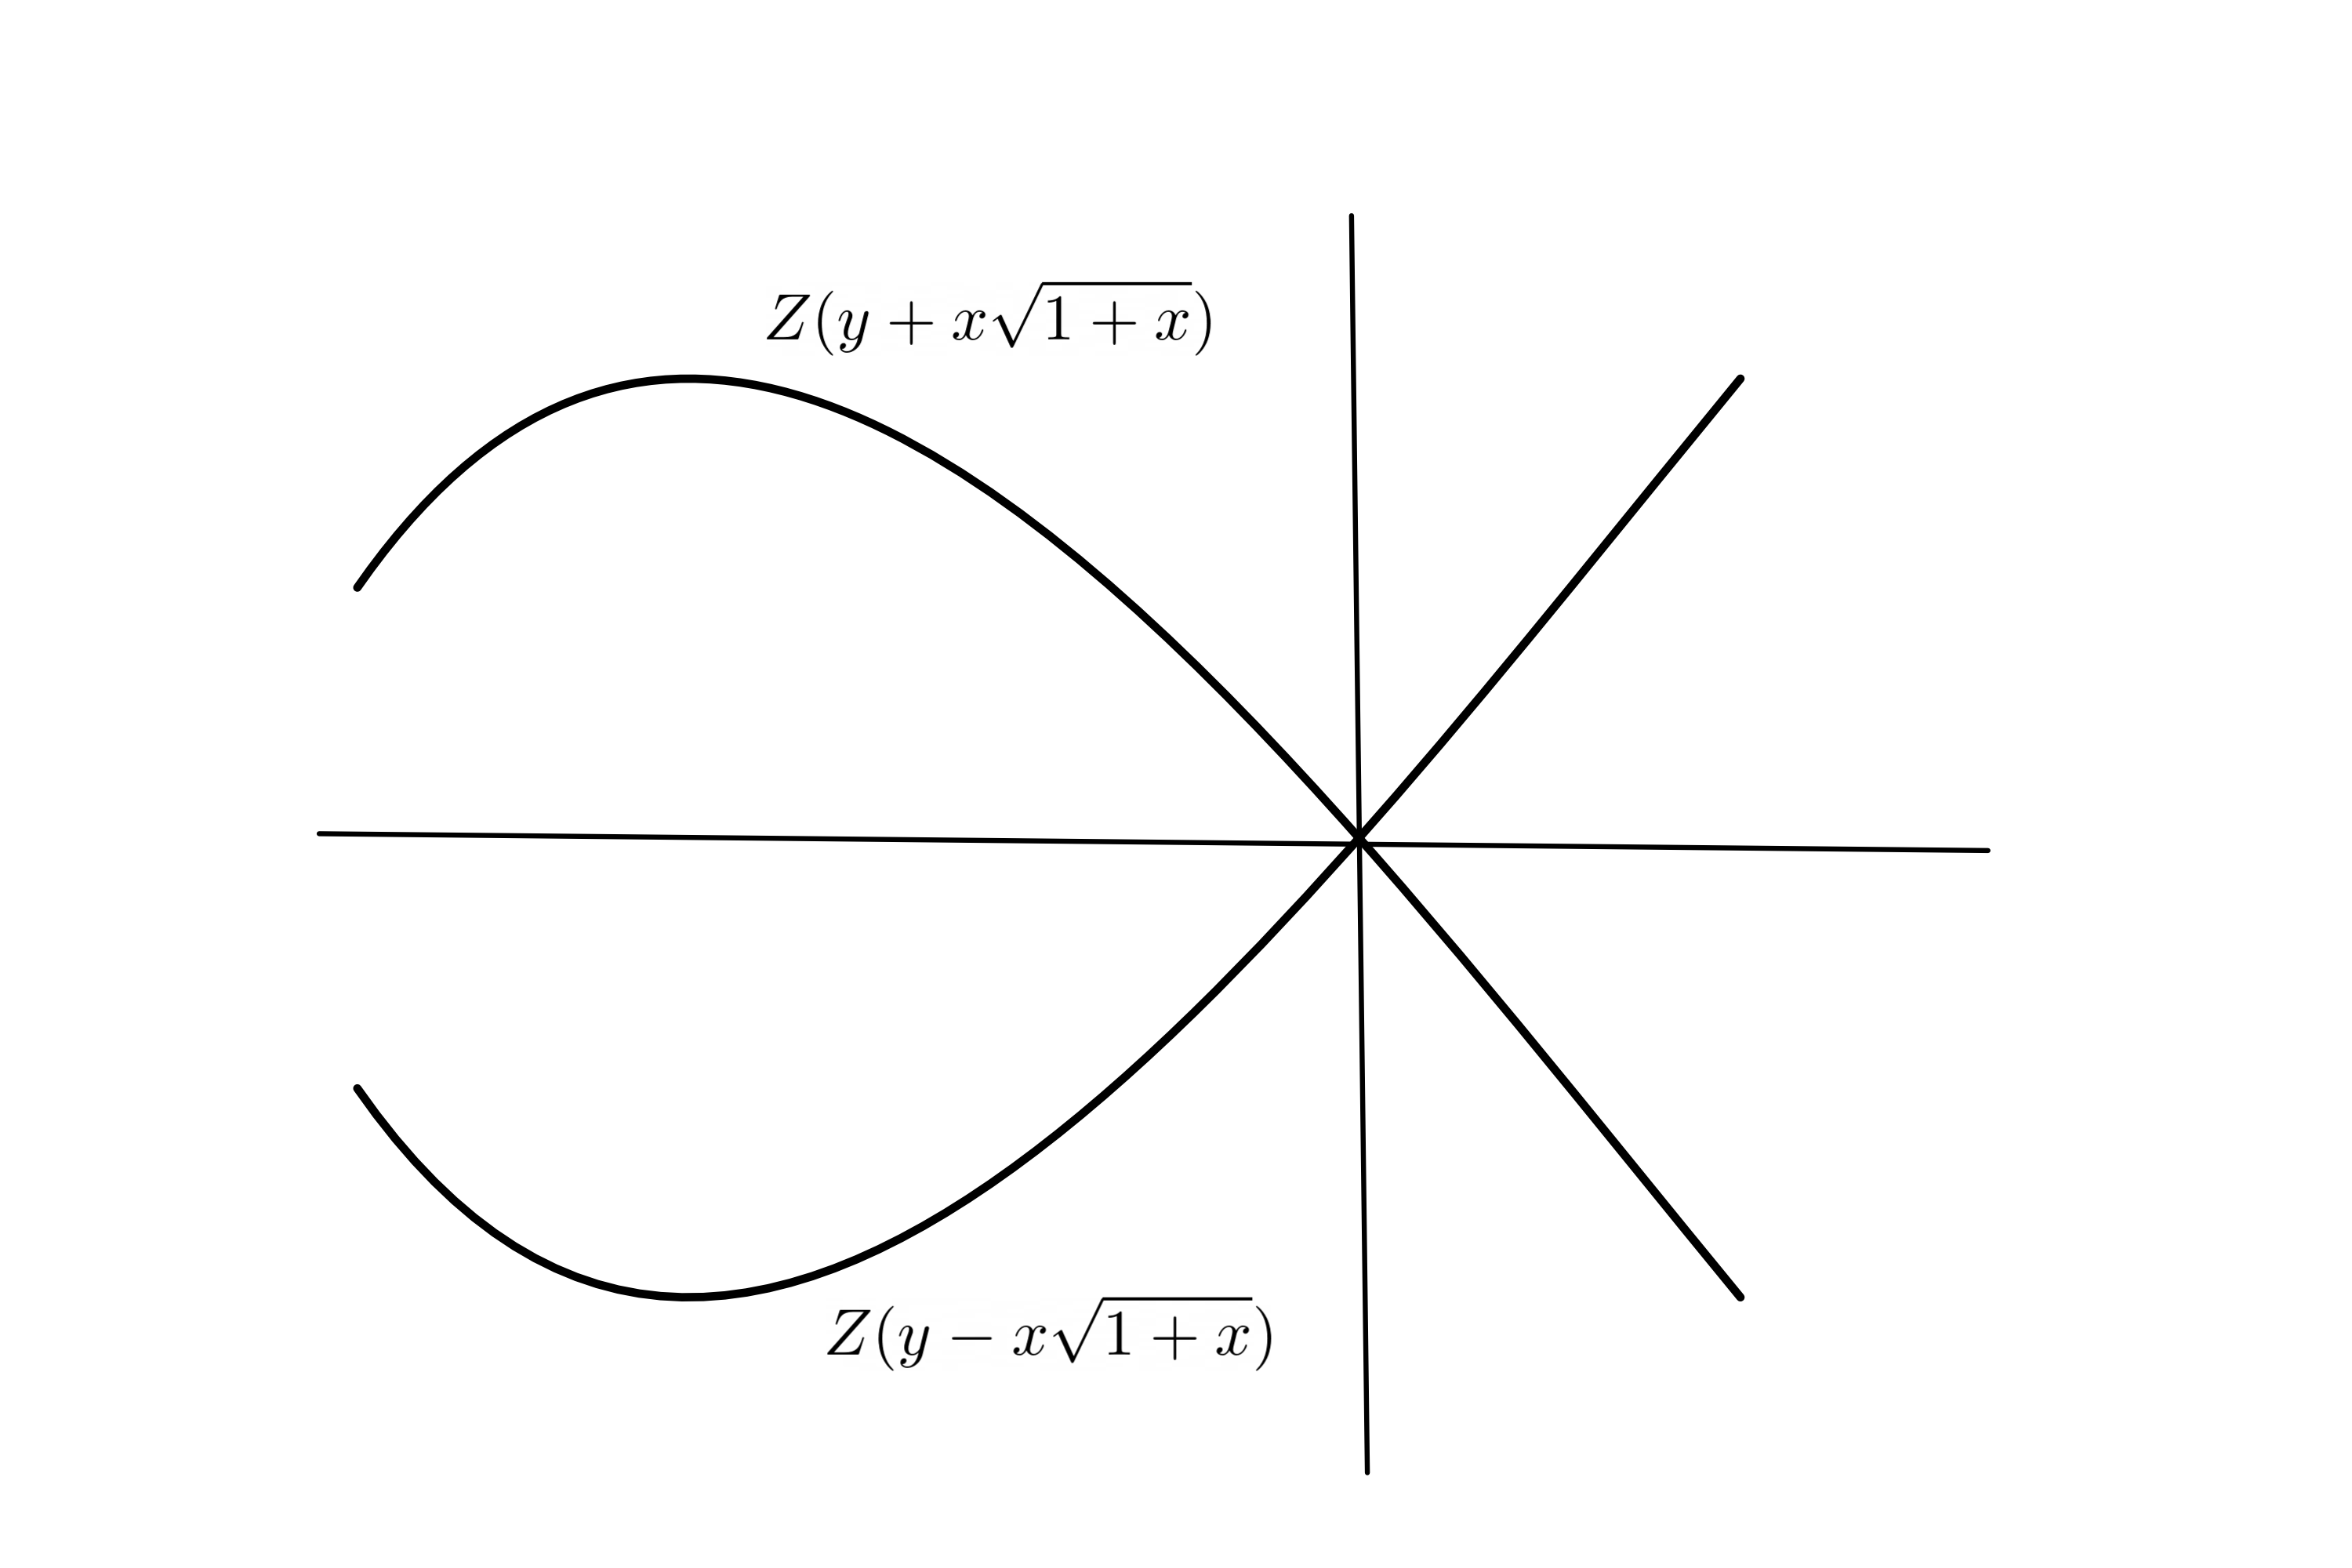
\includegraphics[width=0.5\linewidth]{Imagenes/componenteslocales}
    		\caption{Componentes irreducibles locales de $Z(y^2-x^2-x^3)$.}
    		\label{fig:componenteslocales}
    	\end{figure}
    	
    \end{example}
    
    Por último, presentaremos uno de los resultados más importantes de las subvariedades analíticas:
    
    \begin{theorem}\parencite[Chap 0, Sec. 2.2]{griffiths}\label{irreducibleconexo}
    	Sea $M$ una variedad compleja y $V\subset M$ un subconjunto analítico. Entonces $V$ es irreducible si, y solo si, $V^*$ es conexa.
    \end{theorem}
	
    \subsection{Teoremas de Remmert}
		
		Los subconjuntos analíticos son objetos muy importantes en la geometría algebraica y el análisis complejo. Sin embargo, describir su comportamiento es una tarea lejos de ser trivial y llevó a muchos matemáticos a estudiar en profundidad estos objetos.
		
		Los teoremas de \textit{Remmert} describen el comportamiento de los subconjuntos analíticos bajo imágenes y cerradura. El \textit{teorema de la aplicación propia} nos garantiza que la imagen de un subconjunto analítico por una aplicación holomorfa propia es nuevamente un subconjunto analítico, mientras que el \textit{teorema de Remmert-Stein} describe las condiciones para que la cerradura de un subconjunto analítico siga siendo analítico.
		
		Estos resultados son importantes para la teoría de subconjuntos analíticos y funcionan como herramientas esenciales en nuestro entendimiento de los encajes de variedades complejas. Solo nos limitaremos a enunciar ambos teoremas, remitiendo al lector a las referencias clásicas para entender sus demostraciones (véase \parencite{griffiths}, \parencite{lojasiewicz} y \parencite{chirka}). 
		
    	\begin{theorem}[de la aplicación propia de Remmert]\label{aplicacionpropia}
    		Sea $f:M\to N$ una aplicación holomorfa propia\footnote{Recordemos que una aplicación propia es una función continua entre espacios topológicos cuya preimagen de conjuntos compactos es compacta.} entre variedades complejas. Si $V$ es un subconjunto analítico de $M$, entonces $f(V)$ es un subconjunto analítico de $N$.
    	\end{theorem}
    	Una demostración puede consultarse en el libro \parencite[Chap.3~,Sec.2]{griffiths}, donde se basa fuertemente en una versión particular del teorema de Remmert-Stein llamado \textbf{teorema de Extensión de Levi (II)} y muchas técnicas del análisis complejo. Otra demostración, de carácter más geométrico, fue dada por Chirka \parencite[Chap. 4~, Sec.4.4]{chirka}.
    	
		
		\begin{theorem}[de Remmert-Stein para variedades complejas]\label{remmertstein}
			Sea $M$ una variedad compleja conexa de dimensión $n$ y $Z\subset M$ un subconjunto analítico de codimensión menor a $k+1$. Si $V\subset M\setminus Z$ es un subconjunto analítico de codimensión $k$, entonces la cerradura $\overline{V}$ en $M$ es un subconjunto analítico. 
		\end{theorem}
		
		Para probar este teorema se hace una reducción local del mismo. En primer lugar, por la proposición \ref{puntossingulares}, el conjunto de puntos singulares de $Z$ está contenido en un subconjunto analítico propio $Z_1$. Asimismo, los puntos singulares de $Z_1$ están contenidos en un subconjunto analítico propio $Z_2\subset Z_1$. De esta manera, tenemos la siguiente cadena de subconjuntos analíticos
		\begin{equation*}
			Z=Z_0\supset Z_1 \supset Z_2 \supset \cdots 
		\end{equation*}
		con cada $Z_j\setminus Z_{j+1}$ una subvariedad compleja de codimensión $\geq k$ en $M$. Como cada $Z_{j+1}$ es un subconjunto analítico propio de $Z_j$, su dimensión es estrictamente menor, por lo tanto, el proceso termina después de un número finito de pasos. Entonces existe un $r\in\nn$ tal que $Z_{r+1}=\emptyset$. De esta manera, podemos extender $V$ sucesivamente en cada subvariedad $Z_{j}\setminus Z_{j+1}$, primero tomando la cerradura en $M\setminus Z_{1}$, luego en $M\setminus Z_2$ y continuando una cantidad finita de veces. Con lo cual, es suficiente probarlo suponiendo que $Z\subset M$ es una subvariedad compleja de codimensión $\geq k$.
		
		En segundo lugar, para probar que $\overline{V}$ es analítico, es suficiente mostrar que lo es en una vecindad para cualquiera de sus puntos. Por lo tanto, podemos suponer que $M$ es un polidisco de $\cc^n$ que contiene al origen y $0\in Z$. Después de un cambio de coordenadas,  podemos ver que la subvariedad $Z$ es de la forma $Z=Z(z_1,z_2,\dots,z_{k+1})$. De esta manera, tenemos la reducción local del teorema:
		
		\begin{propo}
			Sean $D\subset\cc^n$ un polidisco que contiene al origen y $Z=Z(z_1,z_2,\dots,z_{k+1})$. Si $V$ es un subconjunto analítico de $D\setminus Z$ de codimensión $k$, entonces $\overline{V}$ es un subconjunto analítico de $D$.
		\end{propo}
		
		\begin{remark}
			El teorema de Remmert-Stein puede ser visto como una generalización geométrica del teorema de Hartogs. Una versión del teorema de Hartogs nos dice que si $f$ es una función holomorfa en $M\setminus\{p\}$, y $\dim M\geq 2$, entonces $f$ se extiende holomorficamente a toda $M$ (véase \parencite[Chap. 2, Sec. 1, Cor. 2.1.6]{huybrechts2005complex}).
			
			En esta misma situación, la gráfica
			\begin{equation*}
				\Gamma_f=\{(x,f(x)):x\in M\setminus \{p\}\}\subset (M\setminus \{p\})\times \cc,
			\end{equation*}
			es un subconjunto analítico. Así, el teorema de Remmert-Stein nos dice que la cerradura $\overline{\Gamma_f}$ es un subconjunto analítico de $M\times \cc$. En particular, $\overline{\Gamma_f}$ resulta ser la gráfica de una función holomorfa
			\begin{equation*}
				\tilde{f}\in\oo_M(M)
			\end{equation*}
			tal que $\tilde{f}|_{M\setminus\{p\}}=f$. Este es exactamente el mismo resultado que nos da Hartogs. 
		\end{remark}
		
    \section{Teorema de Chow}
    
	Hemos estudiado las subvariedades analíticas y visto muchas propiedades interesantes de ellas. Para el objetivo de buscar la algebrización de variedades complejas, vimos que las imágenes de subvariedades analíticas son analíticas (\ref{aplicacionpropia}). Así, un encaje de una variedad compleja al espacio proyectivo significa tener un biholomorfismo entre la variedad y una subvariedad analítica del espacio proyectivo. Por lo tanto, la última pregunta que nos interesa abordar resulta tanto natural como profunda. ¿Cómo son las subvariedades analíticas del espacio proyectivo?
	
	En 1949, \textit{Wei-Liang Chow} publicó su artículo \enquote{On Compact Complex Analytic Varieties}, en el cual demuestra un profundo resultado conocido actualmente como \textit{teorema de Chow} y responde a las cuestiones más importantes de todo este trabajo. La demostración de este resultado ha tenido una historia y desarrollo muy interesante durante el siglo pasado. El enfoque de Chow fue usar varias técnicas analíticas y topológicas, luego en 1953 Reinhold Remmert y Karl Stein presentaron una demostración más simple desarrollando un resultado relacionado con la cerradura de conjuntos analíticos. Tres años después, en 1956, \textit{Jean Pierre Serre} publicó su famoso artículo \textit{"Géométrie algébrique et géométrie analytique"}, bautizado como \textbf{GAGA}, y presentó una demostración muy elegante usando toda la nueva herramienta de gavillas coherentes que desarrolló en su artículo. En nuestro caso, presentaremos una demostración basada en la construcción de Remmert y Stein.

\begin{theorem}[Teorema de Chow]
	Todo subconjunto analítico del $n$-espacio proyectivo es algebraico.
\end{theorem}
	\begin{proof}\parencite{chirka}
		Sea $X\subset \pp^n$ un subconjunto analítico. Consideremos la proyección usual
		\begin{align*}
			\pi:\cc^{n+1}\setminus\{0\}\longrightarrow \pp^n
		\end{align*}
		Tomando $V_0=\pi^{-1}(X)\subset \cc^{n+1}\setminus\{0\}$, entonces $V_0$ es un subconjunto analítico (\ref{preimagen analitico}) de $\cc^{n+1}\setminus\{0\}$. Por el teorema de Remmert-Stein \ref{remmertstein}, la cerradura 
		\begin{equation*}
			V=\overline{V_0}=V_0\cup\{0\}
		\end{equation*}
		es un subconjunto analítico de $\cc^{n+1}$.\\
		Ahora, observemos que  si $z\in V$, entonces para todo $t\in\cc$ tenemos que $tz\in V$. Esto significa que $V$ es un cono completo.
		
		Como $0\in V$, entonces existe una vecindad $U\subset\cc^{n+1}$ de $0$ y $f_1,\dots,f_k\in\mathscr{O}_{\cc^{n+1}}(U)$ tales que 
		\begin{equation*}
			V\cap U=Z(f_1,\dots,f_k).
		\end{equation*}
		Sea $I=\langle \overline{f_1},\dots,\overline{f_k} \rangle\subset \mathscr{O}_{n+1}$ el ideal de gérmenes. Si $\overline{f}\in I$, entonces $f$ se puede escribir como 
		\begin{equation*}
			f(z)=\sum_{i=0}^{\infty}h_i(z)
		\end{equation*}
		donde $h_i\in\cc[z_0,\dots,z_n]_{(i)}$ son polinomios homogéneos de grado $i$.\\
		Como $V$ es un cono, entonces $\overline{h_i}\in I$ para todo $i$. En efecto, si $z\in V$ y $|\lambda|<1$, entonces 
		\begin{equation*}
			0=f(\lambda z)=\sum_{i=0}^{\infty}h_i(\lambda z)=\sum_{i=0}^{\infty}\lambda^ih_i( z)
		\end{equation*}
		Como $f(\lambda z)$ es holomorfa en $\lambda$, entonces por el teorema de la identidad, $h_i(z)=0$ para todo $i\in\nn$. Con esto, $\overline{h_i}\in I$.\\
		Así, $I$ está generado por polinomios homogéneos. Como $\mathscr{O}_{n+1}$ es noetheriano (véase teorema \ref{anillonoetheriano}), $I$ es finitamente generado. Esto significa que existen $F_1,\dots, F_m\in\cc[z_0,\dots,z_n]$ polinomios homogéneos tal que $I=\langle F_1,\dots, F_m \rangle$.
		Por lo tanto, $X=Z(F_1,\dots,F_m)$.
	\end{proof}
	
	Supongamos que $M$ admite un haz lineal amplio $L\longrightarrow M$, entonces existe un encaje holomorfo a algún espacio proyectivo $\varphi:M\hookrightarrow\pp^N$
	\[\begin{tikzcd}
		L \\
		\\
		M && {\mathbb{P}^N}
		\arrow[no head, from=1-1, to=3-1]
		\arrow[hook, from=3-1, to=3-3]
	\end{tikzcd}\]
	Como $\varphi$ es un encaje, $\varphi(M)$ es biholomorfo a $M$. Por el teorema de la aplicación propia (\ref{aplicacionpropia}), $\varphi(M)\subset\pp^N$ es una subvariedad analítica. Por el teorema de Chow, $\varphi(M)$ es una variedad algebraica. Por lo tanto, podemos concluir que:

\begin{corollary}
	Toda variedad compleja que admite un haz amplio es algebraica.
\end{corollary}

	Como observamos en el capítulo \ref{cap2}, en geometría compleja no existe un resultado general análogo al teorema de Whitney. Por ello, resulta natural buscar encajes en un espacio tan familiar y estructurado como lo es el espacio proyectivo complejo \(\mathbb{P}^N\). Sin embargo, el teorema de Chow nos muestra que la posibilidad de realizar una variedad compleja como subvariedad proyectiva es una propiedad exclusiva de las variedades algebrizables.
	
	En geometría algebraica, una variedad proyectiva se entiende como una subvariedad algebraica del espacio proyectivo. En nuestra definición, toda variedad proyectiva admite un encaje en un espacio proyectivo complejo; por el Teorema \ref{proyectivossiamplio}, dicha variedad es algebraica. Por lo tanto, nuestra definición de variedad proyectiva coincide con la noción clásica de la geometría algebraica.

	\begin{corollary}\label{teoriemann}
		Toda superficie de Riemann compacta es algebraica.
	\end{corollary}
	
	Con ello observamos que toda superficie de Riemann compacta puede realizarse como una variedad algebraica de dimensión $1$, es decir, como una curva algebraica. Sin embargo, estos resultados son solo teórico y no constituyen, por sí mismos, un método directo para determinar ecuaciones explícitas de una variedad compleja. De hecho, existe una rama activa de las matemáticas dedicada precisamente a construir y estudiar ecuaciones asociadas a superficies de Riemann; un ejemplo clásico de esta perspectiva es la teoría de las curvas modulares.
	
	\begin{example}\parencite{curvaselipticas}
		Consideremos la superficie de Riemann
		\[
		T=\cc/\Lambda,
		\]
		donde $\Lambda=\omega_1\zz+\omega_2\zz$ es una retícula de $\cc$. A este retículo le asociamos la \textbf{función de Weierstrass} $\wp$, que desciende a una función meromorfa en $T$ y está dada por
		\[
		\wp(z)=\frac{1}{z^2}+\sum_{\omega\in\Lambda\setminus\{0\}}
		\left(\frac{1}{(z-\omega)^2}-\frac{1}{\omega^2}\right).
		\]
		Su derivada satisface la relación
		\[
		(\wp'(z))^2=4\wp(z)^3-g_2\wp(z)-g_3,
		\]
		donde $g_2$ y $g_3$ son constantes que dependen de $\Lambda$ y vienen dadas por las \textbf{series de Eisenstein}
		\[
		g_2=60\sum_{\omega\in\Lambda\setminus\{0\}}\frac{1}{\omega^4},
		\qquad
		g_3=140\sum_{\omega\in\Lambda\setminus\{0\}}\frac{1}{\omega^6}.
		\]
		Con esto, obtenemos una aplicación holomorfa bien definida
		\[
		\phi:T\longrightarrow \pp^2,\qquad
		z\longmapsto [\wp(z):\wp(z)^2:1],
		\]
		la cual define un encaje holomorfo. Así, se obtiene un biholomorfismo entre el toro $T$ y la curva elíptica dada por la ecuación
		\[
		4y^2=4x^3-g_2x-g_3.
		\]
		En general, se puede probar que toda superficie de Riemann de género $1$ está dada por la ecuación afín
		\begin{equation*}
			y^2=x(x-1)(x-\lambda),\qquad \text{para todo }\ \lambda\in\cc\setminus\{0,1\}. 
		\end{equation*}
	\end{example}

	\begin{example}[Encaje de Segre]
		Consideremos la superficie compleja $M=\pp^1\times\pp^1$ y denotemos por $p_1:M\to \pp^1$ y $p_2:M\to \pp^1$ las proyecciones de $M$. Por el teorema \ref{seccionesproyectivo}, sabemos que
		\begin{equation*}
			H^0(\pp^1,\oo(1))\cong\langle x_0,x_1\rangle, \qquad H^0(\pp^1,\oo(1))\cong\langle y_0,y_1\rangle.
		\end{equation*}
		Además, el pullback de las secciones bajo las proyecciones vuelven a ser los monomios $x_0,x_1,y_0,y_1$. De esta manera, las secciones $x_0$ y $x_1$ son linealmente independientes en $H^0(M,p_1^*\oo(1))$, y análogo con $y_0$ y $y_1$. Por lo que, estas secciones definen un subespacio lineal
		\begin{equation*}
			\cc[x_0,x_1]_{(1)}\otimes \cc[y_0,y_1]_{(1)}=\langle x_0,x_1\rangle\otimes \langle y_0,y_1\rangle\subset H^0(M,p_1^*\oo(1))\otimes H^0(M,p_2^*\oo(1)).
		\end{equation*}
		Definamos el haz lineal $L=p_1^*\oo(1)\otimes p_2^*\oo(1)$. Entonces, las secciones
		\begin{equation*}
			x_0\otimes y_0,\enspace x_0\otimes y_1,\enspace x_1\otimes y_0,\enspace x_1\otimes y_1
		\end{equation*}
		definen secciones linealmente independientes de $H^0(M,L)$. Usando el isomorfismo
		\begin{align*}
			\cc[x_0,x_1]\otimes \cc[y_0,y_1]\cong \cc[x_0,x_1,y_0,y_1]
		\end{align*}
		obtenemos que los productos 
		\begin{equation*}
			x_0y_0,\enspace x_0y_1,\enspace x_1y_0,\enspace x_1y_1
		\end{equation*}
		definen secciones linealmente independientes de $H^0(M,L)$. Con lo cual, obtenemos el morfismo inducido por estas secciones
		\begin{align*}
				&\sigma:\pp^1\times\pp^1\longrightarrow \pp^3\\
			([x_0:x_1],[y_0:&y_1])\mapsto [x_0y_0:x_0y_1:x_1y_0:x_1y_1]
		\end{align*}

		Notemos que la aplicación $\sigma$ es holomorfa, pues sus coordenadas homogéneas son productos de coordenadas homogéneas en cada factor. Para probar que $\sigma$ es un encaje holomorfo, estudiaremos su expresión en cartas afines. Consideremos las cartas estándar de $\pp^1$
		\begin{align*}
			&U_0=\{[x_0:x_1]:x_0\neq 0\},\qquad U_1=\{[x_0:x_1]:x_1\neq 0\},\\
			&V_0=\{[y_0:y_1]:y_0\neq 0\},\qquad V_1=\{[y_0:y_1]:y_1\neq 0\}.
		\end{align*}
		En $U_0\times V_0$ tenemos las coordenadas afines $(s,t)$ donde
		\begin{equation*}
			s=\frac{x_1}{x_0},\qquad t=\frac{y_1}{y_0}.
		\end{equation*}
		Dado que 
		\begin{equation*}
			[x_0y_0:x_0y_1:x_1y_0:x_1y_1]=\left[ 1:\frac{y_1}{y_0}:\frac{x_1}{x_0}:\frac{x_1y_1}{x_0y_0}\right],
		\end{equation*}
		entonces en las coordenadas $(s,t)$ la aplicación $\sigma$ queda dada como
		\begin{equation*}
			(s,t)\longmapsto [1:t:s:st].
		\end{equation*}
		Por tanto, sobre la carta afín $Z(X_0)^c\subset\pp^3$, la inversa de $\sigma$ sobre su imagen viene dada por
		\begin{equation*}
			[X_0:X_1:X_2:X_3]\longmapsto \left([1:X_2/X_0],[1:X_1/X_0]\right),
		\end{equation*}
		la cual es holomorfa. Análogamente, en las otras tres cartas de $M$ se obtienen expresiones locales de $\sigma$ y de su inversa dadas por
		\begin{align*}
			&U_0\times V_1:\quad (s,t)\mapsto [t:1:st:s],\qquad
			[X]\mapsto \left([1:X_3/X_1],[X_0/X_1:1]\right),\\
			&U_1\times V_0:\quad (s,t)\mapsto [s:st:1:t],\qquad
			[X]\mapsto \left([X_0/X_2:1],[1:X_3/X_2]\right),\\
			&U_1\times V_1:\quad (s,t)\mapsto [st:s:t:1],\qquad
			[X]\mapsto \left([X_1/X_3:1],[X_2/X_3:1]\right).
		\end{align*}
		De aquí se sigue que $\sigma$ induce un biholomorfismo entre $M=\pp^1\times\pp^1$ y su imagen.
		
		Más aún, la imagen de $\sigma$ es la variedad algebraica proyectiva
		\begin{equation*}
			\sigma(M)=Z(X_0X_3-X_1X_2).
		\end{equation*}
		De esta manera, por la proposición \ref{encajesubvariedades}, la aplicación $\sigma$ es un encaje holomorfo.
		
		Por lo tanto, la superficie compleja $M=\pp^1\times\pp^1$ es algebrizable y la variedad algebraica asociada es
		\begin{equation*}
			V=Z(X_0X_3-X_1X_2)\subset\pp^3,
		\end{equation*}
			
%			Resta identificar la imagen. Si
%			\[
%			[X_0:X_1:X_2:X_3]=\sigma([u_0:u_1],[v_0:v_1]),
%			\]
%			entonces
%			\[
%			X_0X_3-X_1X_2
%			=
%			(u_0v_0)(u_1v_1)-(u_0v_1)(u_1v_0)=0,
%			\]
%			luego \(\sigma(\PP^1\times \PP^1)\subseteq V(X_0X_3-X_1X_2)\).
%			
%			Recíprocamente, si \([X_0:X_1:X_2:X_3]\in V(X_0X_3-X_1X_2)\), entonces la matriz
%			\[
%			\begin{pmatrix}
%				X_0 & X_1\\
%				X_2 & X_3
%			\end{pmatrix}
%			\]
%			tiene determinante cero, y por tanto rango a lo más uno. En consecuencia, dicha matriz se descompone como producto exterior de dos vectores no nulos de \(\CC^2\), es decir, existen \((u_0,u_1)\neq (0,0)\) y \((v_0,v_1)\neq (0,0)\) tales que
%			\[
%			\begin{pmatrix}
%				X_0 & X_1\\
%				X_2 & X_3
%			\end{pmatrix}
%			=
%			\begin{pmatrix}
%				u_0\\
%				u_1
%			\end{pmatrix}
%			\begin{pmatrix}
%				v_0 & v_1
%			\end{pmatrix}.
%			\]
%			Por lo tanto,
%			\[
%			[X_0:X_1:X_2:X_3]
%			=
%			[u_0v_0:u_0v_1:u_1v_0:u_1v_1]
%			\in \sigma(\PP^1\times\PP^1).
%			\]
%			Así,
%			\[
%			\sigma(\PP^1\times\PP^1)=V().
%			\]
%			

	\end{example}

\section{Otros criterios de algebrización}

En esta última sección presentaremos dos conceptos clave en la geometría compleja: las variedades de Moishezon y las variedades de Kähler. Ambos están profundamente relacionados con el problema de la algebrización. Sin embargo, para estudiarlos detalladamente necesitamos desarrollar herramientas más avanzadas que las desarrolladas hasta ahora.

La teoría de Moishezon se apoya en las funciones y aplicaciones meromorfas, las cuales surgen como un análogo a las funciones racionales y equivalencia birracional de la geometría algebraica. Por otro lado, la teoría de Kähler involucra técnicas de geometría diferencial, como métricas riemannianas, formas diferenciales, formas holomorfas y teorías de cohomología.

El objetivo no es desarrollar en profundidad estas teorías, sino presentar su importancia en la algebrización. Mientras que el trabajo de Moishezon estableció una relación muy profunda entre la geometría compleja con la algebraica, las variedades de Kähler lo hacen desde la geometría diferencial. De esta manera, esta sección funciona como una extensión conceptual del trabajo, orientada a mostrar conexiones con resultados más profundos de la geometría compleja.

\subsection{Variedades de Moishezon}

En geometría diferencial o algebraica, es común estudiar el comportamiento global de los objetos estudiando sus funciones. Sin embargo, notamos que las funciones holomorfas sobre variedades complejas conexas compactas (por ejemplo, las superficies de Riemann compactas) son constantes (\ref{holomorfasglobal}). Por lo que no podemos obtener información global de estas variedades a partir de sus funciones ¿Qué podemos hacer?

Las funciones meromorfas extienden el concepto de funciones holomorfas al permitir \enquote{polos controlados}, lo que enriquece aún más la estructura analítica de las variedades. Más aún, el conjunto de todas las funciones meromorfas forma un campo (véase proposición \ref{campodefunciones}), lo cual permite aplicar herramientas algebraicas más potentes. De esta manera, el estudio de las funciones meromorfas se vuelve esencial para comprender la estructura local y la geometría global de las variedades complejas.

\begin{definition}
	Sea $M$ una variedad compleja y $p\in M$. Definamos
	\begin{equation*}
		\mathcal{K}_{M,p}:=Q(\oo_{M,p})
	\end{equation*}
	donde $Q(\oo_{M,p})$ es el campo de fracciones asociado al dominio entero $\oo_{M,p}$ (véase corolario \ref{dominiolocal}). Esto es,
	\begin{equation*}
		\mathcal{K}_{M,p}=\left\{ \frac{f_p}{g_p}:f_p,g_p\in\oo_{M,p}\text{ y }g_p\neq 0\right\}.
	\end{equation*}
	Este campo es llamado \textbf{campo de funciones meromorfas} en $p$.
\end{definition}  

\begin{definition}
	Sea $M$ una variedad compleja. Una \textbf{función meromorfa} sobre $U\subset M$ es una aplicación
	\begin{equation*}
		f:U\longrightarrow \bigsqcup_{x\in U}\mathcal{K}_{M,x}
	\end{equation*}
	la cual asocia a $x\in U$ una función $f_x\in \mathcal{K}_{M,x}$ la cual cumple que para todo $p\in U$, existe una vecindad $V\subset U$ de $p$ y funciones holomorfas $g,h\in\oo_M(V)$, con $h\neq 0$, tal que $f|_V=\frac{g}{h}$\footnote{Esta igualdad significa que para todo $x\in V$ se tiene que $f(x)=\frac{g_x}{h_x}$.}.
\end{definition}

La \textbf{gavilla de funciones meromorfas} se denota por $\mathcal{K}_{M}$ y asigna a cada abierto $U$ el conjunto de funciones meromorfas sobre $U$.

\begin{propo}\label{campodefunciones}
	Sea $M$ una variedad compleja y $U\subset M$ un abierto conexo. Entonces $\mathcal{K}_{M}(U)$ es un campo.
\end{propo}
\begin{proof}
	Recordemos que la estructura de anillo de $\mathcal{K}_{M}(U)$ está dada punto a punto, es decir,
	\begin{align*}
		(f+g)(x):=f(x)+g(x)\in\mathcal{K}_{M,x}\\
		(fg)(x):=f(x)g(x)\in\mathcal{K}_{M,x}.
	\end{align*}
	y el elemento unidad es la función constante $1$ la cual es la fracción $1/1$ en cada campo $\mathcal{K}_{M,p}$.
	
	Sea $f\in \mathcal{K}_{M}(U)$ no cero. Buscamos un $f^{-1}\in\mathcal{K}_{M}(U)$ tal que $ff^{-1}=1$.
	Como $f\neq 0$, entonces existe un punto $p\in U$ tal que $f_p\in\mathcal{K}_{M,p}$ es no cero. Entonces existe una vecindad $V\subset U$ conexa de $p$ tal que
	\begin{equation*}
		f|_V=\frac gh,\qquad g,h\in\oo_M(V),\enspace h\neq 0,\enspace g_p\not\in\mathfrak{m}_p.
	\end{equation*}
	Es decir, $g_p\neq 0$ como germen en $p$. Notemos que el conjunto 
	\begin{equation*}
		Z=\{x\in V:g(x)=0\}
	\end{equation*}
	es un subconjunto analítico propio, esto es, $g$ no se puede anular en un abierto no vacío de $V$. Si $g$ se anulara en todo $V$, entonces $f|_V=0$ y contradice que $f_p\neq 0$.
	
	De esta manera, podemos definir la inversa localmente 
	\begin{equation*}
		f^{-1}|_V=\frac hg.
	\end{equation*} 
	Repetimos este proceso para cada punto donde el germen no sea nulo. Esto nos da una cubierta $\{W_i\}_{i\in I}$ de $U$ tal que
	\begin{equation*}
		f^{-1}|_{W_i}=\frac{h_i}{g_i}
	\end{equation*}
	está bien definida y satisfacen 
	\begin{equation*}
		f|_{W_i}f^{-1}|_{W_i}=1\in\mathcal{K}_M(W_i).
	\end{equation*}
	Notemos que además las funciones $f^{-1}|_{W_i}$ coinciden en las intersecciones $W_i\cap W_j$. Así, por la propiedad de sección global de la gavilla $\mathcal{K}_M$ tenemos que existe $f^{-1}\in \mathcal{K}_{M}(U)$ tal que
	\begin{equation*}
		ff^{-1}=1.
	\end{equation*}
\end{proof}

Si $M$ es una variedad compleja conexa, el espacio de secciones globales $\mathcal{K}_{M}(M)$ es llamado \textbf{campo de funciones meromorfas} sobre $M$ y lo denotamos por $\mathcal{K}(M)$. Este campo es de suma importancia para las variedades complejas y se relaciona con un teorema muy importante de la geometría compleja.

\begin{theorem}[Siegel]
	Sea $M$ una variedad compleja conexa compacta de dimensión $n$. Entonces
	\begin{equation*}
		\mathrm{trdeg}_\cc\mathcal{K}(M)\leq n.
	\end{equation*}
\end{theorem}
Una demostración detallada puede consultarse en \parencite[Teo. 4.23]{carlosga} y está basado en el lema de Schwarz de análisis complejo.

\begin{definition}
	Sea $M$ una variedad compleja conexa compacta. Definimos la \textbf{dimensión algebraica} de $M$ como
	\begin{equation*}
		a(M):=\mathrm{trdeg}_\cc\mathcal{K}(M).
	\end{equation*}
\end{definition}

Por el teorema de Siegel, la dimensión algebraica siempre está acotada por la dimensión de la variedad. Por lo que, la dimensión algebraica puede interpretarse como una medida del grado en que una variedad compleja se aproxima al mundo algebraico.

\begin{theorem}\parencite[Chap. VIII, Sec. 3.1, Theo. 1]{shafarevich2016basic}
	Sea $V\subset \pp^n$ una variedad algebraica no singular. Entonces las funciones meromorfas y funciones racionales en $V$ coinciden. Es decir, $\mathcal{K}(V)=\cc(V)$.
\end{theorem}

Sabemos que en variedades algebraicas, el grado de trascendencia de $\cc(V)$ coincide con la dimensión de la variedad algebraica (véase observación \ref{dimcubierta}). Así, la dimensión algebraica de una variedad algebraica coincide con su dimensión compleja, esto es,
\begin{equation*}
	a(V)=n.
\end{equation*}
Esto último nos lleva a la siguiente definición.

\begin{definition}
	Una variedad compleja conexa compacta $M$ se llama \textbf{variedad de Moishezon} si
	\begin{equation*}
		a(M)=\dim M.
	\end{equation*}
\end{definition}

Su nombre se debe al matemático ruso \textit{Boris Gershevich Moishezon} y sus trabajos publicados en 1966 \enquote{On $n$-dimensional compact varieties with n algebraically independent meromorphic functions, I, II and III} en los cuales introdujo el estudio de estas variedades y desarrolló los resultados que veremos más adelante.

Las variedades algebraicas son ejemplos de variedades de Moishezon y de esta manera, tenemos el siguiente resultado:

\begin{corollary}
	Toda variedad compleja algebrizable es de Moishezon.
\end{corollary}

De esta manera, ser de Moishezon es una condición necesaria para buscar variedades algebrizables. Así, surgen dos preguntas importantes:

\begin{itemize}
	\item ¿Todas las variedades complejas son de Moishezon?
	\item ¿Ser de Moishezon es una condición suficiente para la algebrización?
\end{itemize}
Sin embargo, las respuestas a estas dos preguntas son negativas. Un contraejemplo a la primera cuestión es el siguiente:

\begin{example}[Variedad que no es Moishezon]\label{hopfsuperficie}
	Sea $A:\cc^2\to\cc^2$ la aplicación definida por
	\begin{equation*}
		A(z_1,z_2)=(\lambda z_1,\lambda z_2),\qquad 0<|\lambda|<1.
	\end{equation*}
	Consideremos el grupo cíclico
	\begin{equation*}
		\langle A\rangle=\{A^n:n\in\zz\}.
	\end{equation*}
	Como $A(z)=\lambda z$, entonces
	\begin{equation*}
		A^n(z)=\lambda^n z.
	\end{equation*}
	Así, tenemos la relación de equivalencia
	\begin{equation*}
		z\sim w\qquad \longleftrightarrow\qquad w=A^n(z)\enspace \text{para algún }\ n\in\zz.
	\end{equation*}
	Con lo cual, obtenemos la superficie compleja
	\begin{equation*}
		M=\cc^2\setminus\{0\}/\sim,
	\end{equation*}
	llamada \textbf{superficie de Hopf} (véase \parencite[Example 1.19]{leecomplex}). En particular, $M$ es difeomorfo a $S^1\times S^3$. Sea
	\begin{equation*}
		f\in\mathcal{K}(M)
	\end{equation*}
	una función meromorfa definida en $M$. Tomando el pullback por el cociente $\pi:\cc^2\setminus\{0\}\to M$
	\begin{equation*}
		\tilde{f}:=f\circ\pi,
	\end{equation*}
	levanta $f$ a una función meromorfa en $\cc^2\setminus\{0\}$ y $A$-invariante, es decir, $\tilde{f}\in\mathcal{K}(\cc^2\setminus\{0\})$ y $\tilde{f}\circ A=\tilde{f}$. Vamos a probar que $\tilde{f}$ es constante.\\
	Notemos que el conjunto $\{0\}$ tiene codimensión $2$ sobre $\cc^2$. Sin embargo, los polos de una función meromorfa están contenidos en un conjunto de codimensión $1$. Así, $\tilde{f}$ tiene una singularidad aislada en el cero. Por el teorema de Hartogs, $\tilde{f}$ se extiende holomorficamente a $0$. En particular, $\tilde{f}$ es continua en $0$.
	Sea $z\in \cc^2\setminus\{0\}$, entonces la sucesión $\{A^nz\}=\{\lambda^nz\}$ converge a cero. Por la continuidad de $\tilde{f}$ en el cero tenemos que 
	\begin{equation*}
		\tilde{f}(z)=\tilde{f}(A^nz)\underset{n\to\infty}{\longrightarrow}\tilde{f}(0).
	\end{equation*}
	Esto quiere decir que $\tilde{f}(z)=\tilde{f}(0)$ para todo $z\in \cc^2\setminus\{0\}$, es decir, $\tilde{f}$ es constante. De esta manera, $f$ es una función constante. Por lo tanto,
	\begin{equation*}
		\mathrm{trdeg}_\cc\mathcal{K}(M)=0.
	\end{equation*} 
	y $M$ no es una variedad de Moishezon.
\end{example}

Un resultado que ya intuía Riemann, el cual fue demostrado más tarde, es que toda superficie de Riemann admite funciones meromorfas no constantes. Es decir, si $S$ es una superficie de Riemann compacta se cumple que
\begin{equation*}
	\mathrm{trdeg}_\cc\mathcal{K}(S)\neq 0.
\end{equation*}
Dado que una superficie de Riemann es una variedad compleja de dimensión $1$, entonces por el teorema de Siegel
\begin{equation*}
	\mathrm{trdeg}_\cc\mathcal{K}(S)=1.
\end{equation*}
De esta manera, toda superficie de Riemann es de Moishezon y por el teorema \ref{teoriemann} sabemos que toda superficie de Riemann compacta es algebrizable. Por lo tanto, en dimensión $1$, ser de Moishezon sí es condición suficiente para ser algebrizable. 

Para dimensión dos, la situación es similar.
\begin{theorem}[Kodaira]
	Toda variedad compleja compacta de dimensión 2 con dos funciones meromorfas algebraicamente independientes es algebrizable.
\end{theorem}  
Por lo tanto, en dimensión $2$, ser de Moishezon también es una condición suficiente para admitir una estructura algebraica. Esto nos quiere decir un contraejemplo de una variedad de Moishezon que no sea algebraica lo vamos a encontrar en dimensión $\geq 3$ (véase contraejemplo de Hironaka \ref{hironakaejemplo}).

Un concepto relacionado con las funciones racionales de variedades algebraicas son las aplicaciones birracionales. Vamos a extender esta área de la geometría algebraica a un contexto analítico.

\begin{definition}[Modificación]
	Sea $\Phi:M\to N$ una aplicación holomorfa propia sobreyectiva. Decimos que $\Phi$ es una \textbf{modificación} (propia) si existen dos subconjuntos analíticos $A\subset M$ y $B\subset N$ tales que 
	\begin{enumerate}
		\item $B=\Phi(A)$.
		\item $\Phi|_{M\setminus A}:M\setminus A\to N\setminus B$ es un biholomorfismo. 
		\item $A$ y $B$ tiene codimensión al menos $1$.
		\item $A$ y $B$ son mínimos con las propiedades anteriores.
	\end{enumerate}
	$A$ es llamado \textbf{conjunto excepcional} y $B$ el \textbf{centro} de la aplicación $\Phi$. También se suele decir que $\Phi$ es el \textbf{blow-down} de $X$ a lo largo de $A$.
\end{definition}

Un modificación propia es el análogo de los morfismos birracionales	 propios de geometría algebraica, pues funcionan como un biholomorfismo en \enquote{casi todas partes}. Es decir, existe un subconjunto analítico cerrado y de interior vacío sobre el cual la aplicación deja de ser un biholomorfismo, pero fuera de él, los espacios son localmente idénticos. En particular, la composición de estos morfismos está bien definidos en un conjunto denso.

\begin{example}[Blow up]
	Vamos a considerar el caso del origen en $\cc^n$. Cada punto $z\in \cc^n$ determina una única línea que pasa por el origen, y en consecuencia un punto en $\pp^{n-1}$, excepto cuando $z=0$. De esta manera, se define
	\begin{equation*}
		\mathrm{Bl}_0\cc^n=\{(z,l)\in\cc^n\times\pp^{n-1}:z\text{ pertenece a la línea }l\subset\cc^n\}.
	\end{equation*}
	Notemos que es exactamente la misma definición que el espacio total del haz tautológico de $\pp^{n-1}$ pero ahora vamos a considerar la proyección a la primera entrada.	
	
	Decimos que $\mathrm{Bl}_0\cc^n$ es el \textbf{blow-up} de $\cc^n$ en el origen y el conjunto $E=\Phi^{-1}(0)$ es llamado \textbf{divisor excepcional}.
	
	Sea $K\subset\cc^n$ un conjunto compacto, entonces
	\begin{equation*}
		\Phi^{-1}(K)=K\times \pp^{n-1}.
	\end{equation*}
	Como el producto de compactos es compacto, entonces $\Phi^{-1}(K)$ es un conjunto compacto. Por lo que, $\Phi$ es una aplicación propia. Notemos además que
	\begin{equation*}
		E=\{(0,l)\in\cc^n\times\pp^{n-1}:l\in\pp^{n-1}\}=\{0\}\times\pp^{n-1},
	\end{equation*}
	el cual es una subvariedad analítica de $\cc^n\times\pp^{n-1}$. Más aún, $E$ tiene codimensión $1$. Luego, el centro es
	\begin{equation*}
		B=\Phi(E)=\{0\}\subset\cc^n
	\end{equation*}
	es una subvariedad analítica de codimensión $n$.
	
	Notemos además que
	\begin{equation*}
		\Phi|_{\mathrm{Bl}_0\cc^n\setminus E}:\mathrm{Bl}_0\cc^n\setminus E\longrightarrow \cc^n\setminus\{0\}
	\end{equation*}
	es biyectiva por definición. Además, es holomorfa por ser una proyección y su inversa viene dada por
	\begin{equation*}
		z\mapsto (z,[z]),
	\end{equation*}
	la cual también es holomorfa. Por lo tanto, $\Phi:\mathrm{Bl}_0\cc^n\to \cc^n$ es una modificación propia.\\
	Sabemos que el morfismo
	\begin{align*}
		&f:\cc^n\dashrightarrow \pp^{n-1}\\
		(z_1,\dots &,z_n)\mapsto [z_1:\cdots:z_n]
	\end{align*}
	no está bien definido en el cero. Sin embargo, se puede factorizar por la proyección a la segunda entrada $\pi:\mathrm{Bl}_0\cc^n\to \pp^{n-1}$, la cual es holomorfa, y el blow-up de la siguiente manera  
	\begin{center}
		\begin{tikzcd}
			& {\mathrm{Bl}_0\mathbb{C}^n} & \\
			\\
			{\mathbb{C}^n} && {\mathbb{P}^{n-1}}
			\arrow["\Phi"', from=1-2, to=3-1]
			\arrow["\pi", from=1-2, to=3-3]
			\arrow["f"', from=3-1, to=3-3]
		\end{tikzcd}
	\end{center}
	En geometría algebraica, a este proceso se le llama \textbf{eliminación de indeterminaciones}.
	\begin{figure}[H]
		\centering
		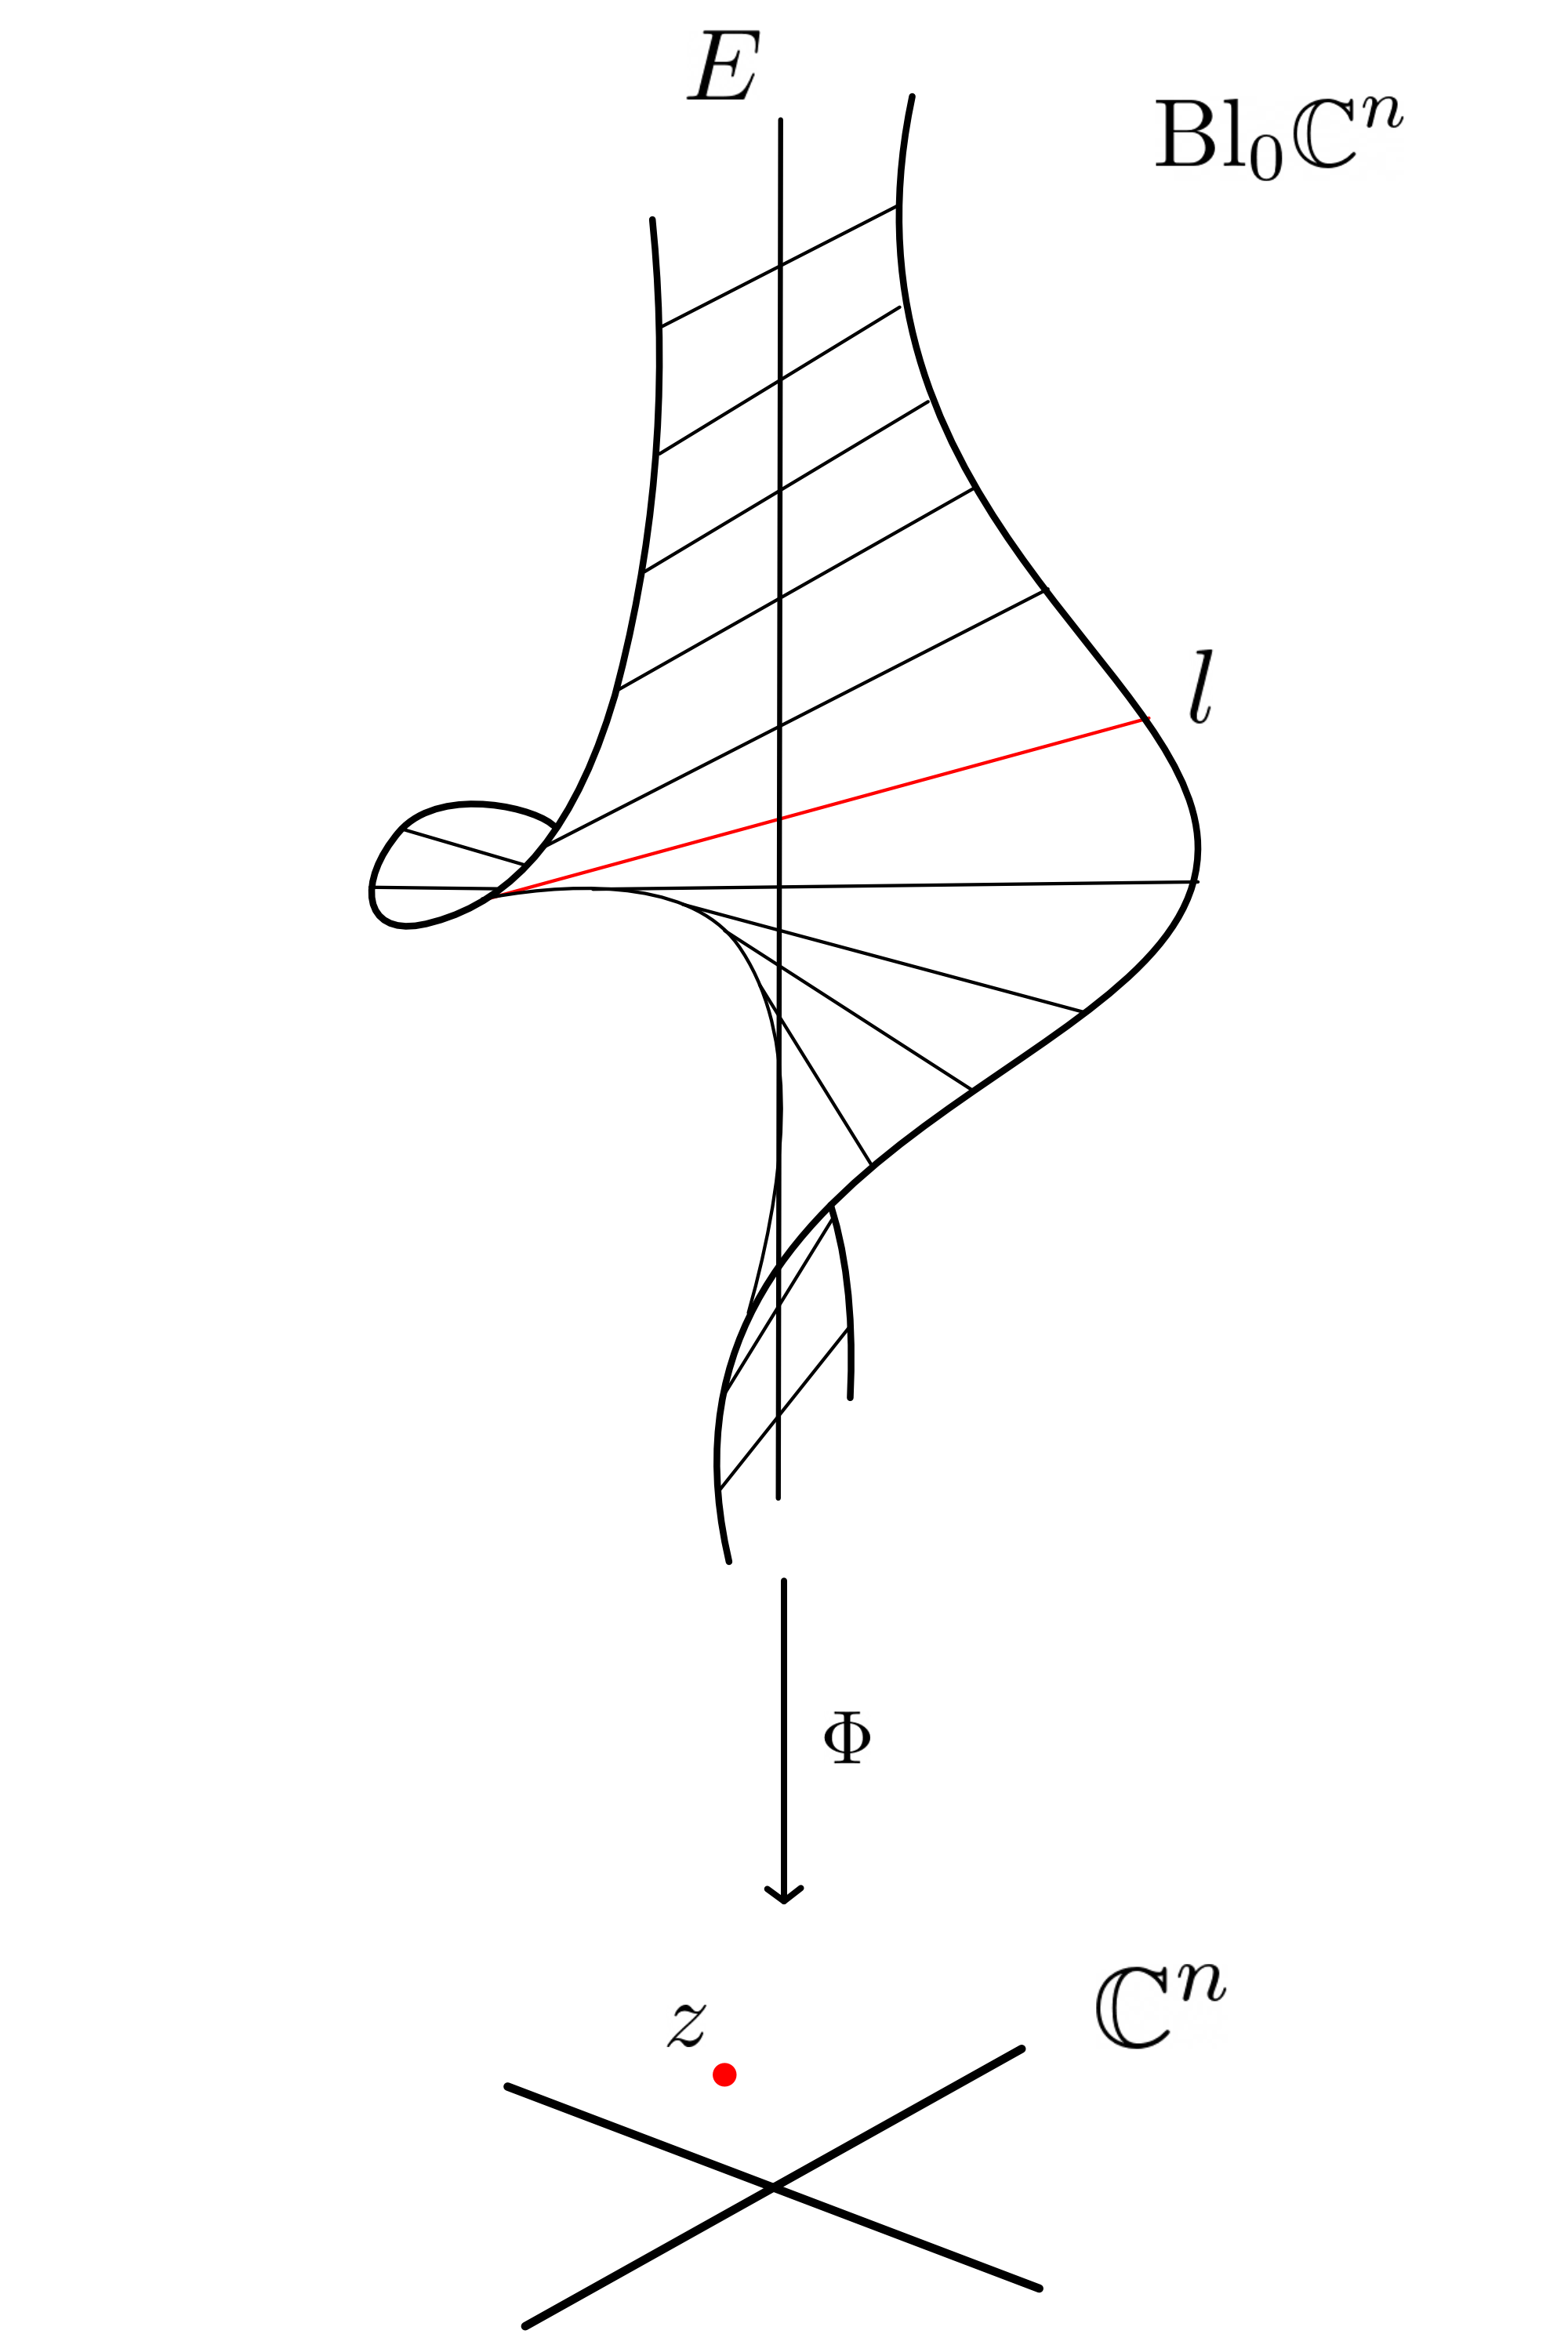
\includegraphics[width=0.45\linewidth]{Imagenes/exposion}
		\caption{Interpretación geométrica del blow-up}
		\label{fig:exposion}
	\end{figure}
	
\end{example}

Las modificaciones son los \enquote{morfismos elementales} de la geometría bimeromorfa, esto debido a que preservan las funciones meromorfas:

\begin{propo}\parencite[Chap VII, Sec. 1, Prop. 1.3]{grauertremment}
	Sea $\Phi:M\to N$ una modificación propia.
	\begin{enumerate}
		\item La aplicación canónica $\widehat{\Phi}:\oo_N\to \Phi_*(\oo_M)$ es un morfismo de gavillas inyectivo.
		\item La aplicación canónica $\widetilde{\Phi}:\mathscr{K}_N\to\Phi_*\mathscr{K}_M$ es un isomorfismo de gavillas.
	\end{enumerate}
	En particular, $\Phi$ induce un isomorfismo de campos $\mathscr{K}(M)\cong\mathscr{K}(N)$.
\end{propo}

\begin{definition}
	Sea $M$ y $N$ variedades complejas. Decimos que una aplicación
	\begin{equation*}
		f:M\dashrightarrow N
	\end{equation*}
	es dice \textbf{meromorfa} si cumple que
	\begin{enumerate}
		\item Existe un subconjunto analítico $A\subset M$ de codimensión al menos $1$ tal que $f$ está bien definido y holomorfo sobre el conjunto abierto denso $U=M\setminus A$. Este conjunto es llamado \textbf{conjunto de indeterminación}.
		\item La cerradura de la gráfica
		\begin{equation*}
			\Gamma_f := \{(x,y)\in U\times N : y=f(x)\}\subset M\times N
		\end{equation*}
		es una subvariedad analítica.
		\item La proyección a la primera coordenada $\Gamma_f\to M$ es una modificación propia.
	\end{enumerate}
	Decimos que $f$ es un \textbf{bimeromorfismo} si existe otra aplicación meromorfa $g:N\dashrightarrow M$ tal que
	\begin{align*}
		f\circ g= id_N,\\
		g\circ f= id_M.
	\end{align*}
	En este caso decimos que $M$ es \textbf{bimeromorfa} a $N$.
\end{definition}

Una aplicación meromorfa $f:M\dashrightarrow N$ puede interpretarse como una aplicación holomorfa después de resolver las indeterminaciones. Específicamente si tomamos las proyecciones
\begin{equation*}
	p_M:\Gamma_f\longrightarrow M\qquad\text{y}\qquad p_N:\Gamma_f\longrightarrow N
\end{equation*}
entonces
\begin{equation*}
	f=p_N\circ p_M^{-1}.
\end{equation*}
Es decir, $f$ se factoriza por una modificación propia. 

De esta manera, $f:N\dashrightarrow M$ es holomorfo casi en todas partes y su gráfica define un subvariedad analítica \enquote{bien comportada} en $M\times N$. La parte \enquote{meromorfa} consiste precisamente en permitir un conjunto de indeterminación de codimensión $\geq 1$, donde no hay una función bien definida.

\begin{remark}\parencite[Chap VII, Sec. 1]{grauertremment}
	Algunos hechos importantes de estas aplicaciones son los siguientes:
	\begin{enumerate}
		\item Si $L$ es un haz lineal sobre $M$, entonces la aplicación inducida
		\begin{equation*}
			\varphi_L:M\longrightarrow\pp^N
		\end{equation*}
		es una aplicación meromorfa, donde el conjunto de indeterminación es $Bs(L)$.
		\item (Teorema de eliminación de indeterminaciones) Sea $f:M\dashrightarrow N$ una aplicación meromorfa. Entonces existe una modificación propia $\sigma:\tilde{M}\to M$ y una aplicación holomorfa $\tau:\tilde{M}\to N$ tal que el siguiente diagrama conmuta
		\begin{center}
			\begin{tikzcd}
				& {\tilde{M}} & \\
				\\
				M && N
				\arrow["\sigma"', from=1-2, to=3-1]
				\arrow["\tau", from=1-2, to=3-3]
				\arrow["f"', from=3-1, to=3-3]
			\end{tikzcd}
		\end{center}
		\item Toda modificación propia es bimeromorfismo.
		\item Toda modificación propia $\Phi:M\to N$ entre superficies complejas compactas es la composición de una cantidad finita de blow-ups en un solo punto.
		\item Toda aplicación bimeromorfa $f:M\dashrightarrow N$ entre variedades complejas compactas puede escribirse como una composición $f=f_1\circ\cdots\circ f_k$ donde $f_i$ son blow-up en un punto o la inversa de un blow-ups en un punto. A la composición de un blow-up con su inversa suele ser llamado \textbf{transformación monoidal}.
	\end{enumerate}
\end{remark}

Análogo al caso de geometría algebraica, si $f:M\dashrightarrow N$ es una aplicación bimeromorfa, entonces induce un isomorfismo de campos
\begin{equation*}
	\mathcal{K}(N)\cong \mathcal{K}(M).
\end{equation*}
Eso significa que
\begin{equation*}
	a(N)=a(M).
\end{equation*}
Por lo tanto, la dimensión algebraica es un invariante bimeromorfo. 

\begin{theorem}[de Moishezon]\parencite{Moishezonlemmachow}
	Sea $M$ una variedad de Moishezon, entonces existe una aplicación bimeromorfa $f:M\dashrightarrow V$ donde $V$ es una variedad algebraica. Es decir, $M$ es bimeromorfa a una variedad algebraica.
\end{theorem}

Este teorema, con un sabor idéntico al \textit{lema de Chow}, muestra una naturaleza algebraica de ciertas variedades complejas. Además, orienta el estudio de la geometría compleja hacia la combinación de técnicas analíticas, birracionales y algebraicas. 

\begin{remark}\parencite[Chap. VII, Sec. 6.4]{grauertremment}\label{espaciosdemoishezon}
	Un \textbf{espacio complejo} (o espacio analítico complejo) es un espacio localmente anillado $(X,\oo_X)$ tal que $X$ es Hausdorff y para cada punto $x\in X$ existe una vecindad $U$ isomorfa a un subconjunto analítico abierto de $\cc^n$, es decir, el espacio localmente anillado $(U,\oo_X|_U)$ es isomorfo a espacio localmente anillado $(Y,\oo_Y)$ donde $Y$ es el abierto
	\begin{equation*}
		Y=\{x\in \Omega\subset\cc^n:f_1(x)=\cdots=f_k(x)=0\}
	\end{equation*}
	junto a la gavilla cociente definida por
	\begin{equation*}
		\oo_Y=\oo_\Omega/\langle f_1,\dots, f_k\rangle,
	\end{equation*}
	restringida a la topología de $Y$.
	
	Los espacios complejos generalizan a las variedades complejas, admitiendo singularidades y elementos nilpotentes en su gavilla. Más aún, existe un funtor llamado \textbf{funtor de analitificación}
	\begin{equation*}
		(\_)^{an}:\{\text{esquemas de tipo finito}/\cc\}\to\{\text{espacios analíticos complejos}\},
	\end{equation*}
	el cual le asocia a un esquema $X$ de tipo finito sobre $\cc$ un espacio complejo $X^{an}$. Sin embargo, este funtor no es una equivalencia pues, como hemos visto, existen muchas variedades complejas (o subconjuntos analíticos en general) que no son algebrizables. Un \textbf{espacio de Moishezon} $X$ es un espacio complejo compacto reducido (sin nilpotentes) bimeromorfo a una variedad algebraica, o equivalentemente,
	\begin{equation*}
		a(X)=\dim X.
	\end{equation*}
	Con lo cual, también hemos trabajado en determinar que espacios de Moishezon sí provienen de esquemas proyectivos de tipo finito sobre $\cc$. Por lo tanto, podemos también preguntarnos: ¿Cuáles son los \enquote{objetos algebraicos} que corresponden con espacios de Moishezon (si es que existen)?
	\end{remark}

\subsection{Variedades de Kähler}

En geometría compleja, la geometría diferencial se desarrolla bajo la restricción impuesta por la estructura compleja. El análogo complejo de una métrica riemanniana es una métrica hermitiana, que es compatible con la estructura compleja y permite introducir nociones métricas respetando la holomorfía. Entre ellas, las métricas de Kähler se distinguen por satisfacer una condición diferencial que unifica la geometría riemanniana, simpléctica y compleja, dando lugar a una teoría especialmente rígida y estructurada.

Para trabajar en este contexto diferencial, primero debemos presentar los espacios tangentes a una variedad compleja. Las construcciones están principalmente basadas de los libros \parencite[Sec. 1.2]{huybrechts2005complex} y \parencite[Cap. 1]{leecomplex}. Fijemos $M$ una variedad compleja y $p\in M$. 
\begin{equation*}
	T_{\rr,p}M=\mathrm{gen}_\rr\left\{\frac{\partial}{\partial x_i},\frac{\partial}{\partial y_i}\right\}.
\end{equation*} 
Definamos el endomorfismo
\begin{align*}
	&J:T_{\rr,p}M\longrightarrow T_{\rr,p}M\\
	J\left(\frac{\partial}{\partial x_i}  \right)&=\frac{\partial}{\partial y_i},\qquad J\left(\frac{\partial}{\partial y_i} \right)=-\frac{\partial}{\partial x_i},
\end{align*}
el cual cumple que $J^2=-\mathrm{Id}$. Esta función es llamada \textbf{estructura casi compleja} de $T_{\rr,p}M$. Ahora, consideremos el espacio complexificado
\begin{equation*}
	T_{\cc.p}M=T_{\rr,p}M\otimes \cc,
\end{equation*}
el cual es llamado \textbf{espacio tangente complejo} de $p$. Además, podemos considerar la extensión de la estructura casi compleja al espacio complexificado $J_\cc:T_{\cc.p}M\to T_{\cc.p}M$. De esta manera, tenemos la descomposición
\begin{equation*}
	T_{\cc.p}M=T_{p}^\prime M\oplus T_p^{\prime\prime}M, 
\end{equation*}
donde
\begin{align*}
	&T_{p}^\prime M=\{v\in T_{\cc.p}M: J(v)=iv\},\\		&T_p^{\prime\prime}M =\{v\in T_{\cc.p}M: J(v)=-iv\}.
\end{align*}
En particular, el espacio $T_{p}^\prime M$ es llamado \textbf{espacio tangente holomorfo} y juega el papel del espacio tangente en la geometría compleja. Además, se cumple que
\begin{equation*}
	\dim_{\cc} T_{p}^\prime M=n
\end{equation*}
pues los operadores 
\begin{equation*}
	\frac{\partial }{\partial z_i}=\frac{1}{2}\left( \frac{\partial }{\partial x_i}-i\frac{\partial }{\partial y_i}\right).
\end{equation*}
forman una base para el espacio tangente holomorfo. Más aún, se tiene la siguiente sucesión exacta de $\rr$-módulos
\begin{center}
	\begin{tikzcd}
		0 & {T_{\mathbb{R},p}M} & {T_{\mathbb{C},p}M} & {T_p^\prime M} & 0
		\arrow[from=1-1, to=1-2]
		\arrow[from=1-2, to=1-3]
		\arrow[from=1-3, to=1-4]
		\arrow[from=1-4, to=1-5]
	\end{tikzcd}
\end{center}
Por lo tanto, podemos concluir que
\begin{equation*}
	T_{\mathbb{R},p}M\cong T_p^\prime M
\end{equation*}
\begin{definition}
	Una \textbf{forma hermitiana} es una función $h:T^\prime_pM\times T^\prime_pM\to\cc$ lineal en la primera entrada y 
	\begin{equation*}
		h(v_1,v_2)=\overline{h(v_2,v_1)},\qquad v_1,v_2\in T^\prime_pM.
	\end{equation*}
\end{definition}
De la definición podemos notar es $\cc$-antilineal y $h_p(v,v)\in\rr$ para todo $v\in T^\prime_pM$. Decimos que $h_p$ es \textbf{positiva definida} si $h_p(v,v)>0$ para todo $v\in T^\prime_pM$.

Usando el isomorfismo $T_{\rr,p}M\cong T^\prime_pM$, podemos ver que si $h_p$ es positivo definido se cumple que
\begin{equation*}
	g(v_1,v_2):=\mathrm{Re}h_p(v_1,v_2)=\frac{1}{2}(h_p(v_1,v_2)+h_p(v_2,v_1))
\end{equation*}
es una métrica riemanniana sobre $M$ como variedad suave. Más aún, $h_p$ está definida únicamente por $g_p$.

\begin{definition}
	Una función bilineal $g:T^\prime_pM\times T^\prime_pM\to\rr$ sobre $M$ se dice \textbf{compatible} con $J$ si
	\begin{equation*}
		g(Ju,Jv)=g(u,v),\qquad\text{para todo }u,v\in T_pM.
	\end{equation*}
\end{definition}

Notemos que la estructura casi compleja $J$ actúa como una rotación $90^\circ$ en cada plano complejo del espacio tangente, pero una métrica albitraria no necesariamente respeta este giro. La compatiblidad de $g$ nos dice que medir después de girar por $J$ es lo mismo que girar después de medir. Un cálculo directo muestra que:
\begin{propo}
	Una función $h_p:T^\prime_pM\times T^\prime_pM\to\cc$ es forma hermitiana si, y solo si, $g_p=\mathrm{Re}h_p$ es una métrica riemanniana en $p$ compatible con $J$.
\end{propo}
%\begin{proof}
%	Supongamos que $h_p:T^\prime_pM\times T^\prime_pM\to\cc$ es una forma hermitiana. Definimos $g:T_{\rr,p}M\times T_{\rr,p}M\to\rr$ la función dada por
%	\begin{equation*}
%		g(v_1,v_2)=\mathrm{Re}h_p(v_1,v_2)=\frac{1}{2}(h_p(v_1,v_2)+h_p(v_2,v_1)).
%	\end{equation*}
%	Notemos que $g$ es bilineal, pues
%	\begin{align*}
%		g(\lambda v_1+v_2,v)=\frac{1}{2}(h_p(\lambda v_1+v_2,v)+h_p(v,\lambda v_1+v_2))=\frac12 (\lambda h_p(v_1,v)+h_p(v_2,v)+\overline{\lambda}\overline{h_p(v_1,v)}´+\overline{h_p(v_1,v)})
%	\end{align*}
%	\textcolor{red}{ACABAR EJEMPLO}
%\end{proof}

Esto significa que la forma hermitiana $h_p$ determina de manera única una métrica riemanniana compatible con $J$, y viceversa. 

Considerando la parte imaginaria
\begin{equation*}
	w_p(u,v)=-\mathrm{Im}h_p(u,v)=\frac{i}{2}(h_p(u,v)-h_p(v,u))
\end{equation*}
es una forma bilineal alternante tal que $w_p(u,v)=g_p(u,Jv)$. Más aún, $h_p$ está definida únicamente por $w_p$.

\begin{propo}
	Una función $h_p:T^\prime_pM\times T^\prime_pM\to\cc$ es forma hermitiana si, y solo si, $w_p=-\mathrm{Im}h_p$ es una 2-forma compatible con $J$.	
\end{propo}
%\begin{proof}
%	\textcolor{red}{FALTA DEMOSTRACIÓN}
%\end{proof}

\begin{definition} 
	Una métrica hermitiana $H$ sobre una variedad compleja $M$ es una colección de formas Hermitianas $h_p$ para todo punto $p\in M$.
\end{definition}

De esta manera, una métrica hermitiana $H$ induce una métrica riemanniana $g=\mathrm{Re}H$ y una $2$-forma diferencial real valuada $w=-\mathrm{Im}H$. A esta forma diferencial se le llamada \textbf{forma fundamental} de $H$. Por lo tanto, esta métrica se puede interpretarse como la versión mínima y natural de una métrica riemanniana que respeta la estructura casi compleja.

\begin{propo}
	Toda variedad compleja admite una métrica hermitiana.
\end{propo}
\begin{proof}
	Sea $M$ una variedad compleja y consideremos una métrica riemanniana $g_0$ arbitraria. Definamos otra métrica riemanniana
	\begin{equation*}
		g(u,v)=g_0(u,v)+g_0(Ju,Jv).
	\end{equation*}  
	Notemos que
	\begin{equation*}
		g(Ju,Jv)=g_0(Ju,Jv)+g_0(J^2u,J^2v)=g_0(-u,-v)+g_0(Ju,Jv)=g_0(u,v)+g_0(Ju,Jv)=g(u,v).
	\end{equation*}
	De esta manera, $g$ es compatible con $J$. Por lo tanto, definiendo $w(u,v)=g(u,Jv)$ obtenemos una métrica hermitiana para $M$
	\begin{equation*}
		h(u,v)=g(u,v)-iw(u,v).
	\end{equation*}
\end{proof}                                     

Si $M$ tiene coordenadas $(z^1,\cdots,z^n)$, entonces una dos forma diferencial $\omega$ está dada por
\begin{equation*}
	\omega=\sum_{i<j}w_{ij}(z)dz^i\wedge dz^j,
\end{equation*}
entonces
\begin{equation*}
	d\omega=\sum_{i<j<k}\left( \frac{\partial w_{jk}}{\partial z_i}+\frac{\partial w_{ki}}{\partial z_j}+\frac{\partial w_{ij}}{\partial z_k}\right)dz^i\wedge dz^j\wedge dz^k.
\end{equation*}
Decimos que $w$ es cerrada si $d\omega=0$.

\begin{definition}
	Una \textbf{variedad de Kähler} es una variedad compleja equipada con una métrica Hermitiana $H$ cuya forma fundamental $\omega=-\mathrm{Im}H$ es cerrada, esto es,
	\begin{equation*}
		d\omega=0.
	\end{equation*}
	En este caso, la forma fundamental $w$ es llamada \textbf{forma de Kähler}.
\end{definition}

La forma fundamental $w$ puede interpretarse como una medida de áreas compatibles con la estructura compleja, por lo que pedir que sea cerrada nos dice que esas áreas complejas no varían infinitesimalmente al moverse en la variedad. Así, la métrica $g$ y la forma $w$ nos respetan los ángulos y áreas a un nivel complejo, es decir, son compatibles con la estructura compleja tanto desde el punto de vista métrico como simpléctico.

Veamos ahora unos ejemplos importantes de variedades de Kähler, los cuales nos ayudarán a entender el caso de algebrización.

\begin{example}
	Consideremos $\cc^n$ con la métrica donde $\frac{\partial}{\partial z_j}$ forman una base unitaria. La estructura casi compleja $J$ actúa sobre los vectores tangentes como
	\begin{equation*}
		J\frac{\partial}{\partial x_j}=\frac{\partial}{\partial y_j},\quad
		J\frac{\partial}{\partial y_j}=-\frac{\partial}{\partial x_j}.
	\end{equation*}
	La métrica euclidiana estándar en $\mathbb{C}^n\simeq\mathbb{R}^{2n}$ es
	\begin{equation*}
		g=\sum_{j=1}^n (dx_j\otimes dx_j+dy_j\otimes dy_j).
	\end{equation*}
	Por otro lado,
	\begin{equation*}
		\omega(u,v)=g(u,Jv).
	\end{equation*}
	En coordenadas, usando que $J$ envía $\partial/\partial x_j\mapsto\partial/\partial y_j$, se obtiene
	\begin{equation*}
		\omega=\sum_{j=1}^n dx_j\wedge dy_j=\frac{i}{2}\sum_{j=1}^{n} dz_i\wedge d\overline{z}_j.
	\end{equation*}
	Como $\omega$ tiene coeficientes constantes, su diferencial exterior es
	\begin{equation*}
		d\omega=\sum_{j=1}^n d(dx_j\wedge dy_j)=
		\sum_{j=1}^n (d dx_j)\wedge dy_j - dx_j\wedge d dy_j=0,
	\end{equation*}
	porque $d (dx_j)=d (dy_j)=0$ para diferenciales exactos de coordenadas. Así que
	\begin{equation*}
		d\omega=0\quad\text{en todo}\qquad \mathbb{C}^n.
	\end{equation*}
	Por lo tanto, $\cc^n$ es una variedad de Kähler.
\end{example}

\begin{example}
	Sea $N\subset M$ una subvariedad compleja. Para todo $p\in N$ se cumple que $T_p^\prime N\subset T_p^\prime M$, entonces una métrica Hermitiana $H_M$ induce naturalmente una métrica en $N$. Calculando en coordenadas locales, se cumple que
	\begin{equation*}
		w_N=i^*w_M
	\end{equation*}
	donde $i:N\hookrightarrow M$ es la aplicación inclusión. Por lo tanto, si $M$ es de Kähler, entonces $N$ también lo es.
\end{example}

\begin{example}[Métrica de Fubini-Study]
	Consideremos el $n$-espacio proyectivo $\pp^n$ y la carta afín
	\begin{equation*}
		U_0=\{[Z_0:\cdots:Z_n]:Z_0\neq 0\}\subset\pp^n.
	\end{equation*}
	con coordenadas locales
	\begin{equation*}
		z_i=\frac{Z_i}{Z_0}.
	\end{equation*} 
	Definamos la función
	\begin{equation*}
		\varphi(z)=\log(1+\|z\|^2)=\log(1+|z_1|^2+\cdots+|z_n|^2).
	\end{equation*}
	llamada \textbf{potencial de Kähler} de la forma 
	\begin{equation*}
		\omega_{FS}=\frac{i}{2\pi}\partial \overline{\partial}\varphi.
	\end{equation*}
	La métrica hermitiana está dada por
	\begin{equation*}
		h_p\left(\frac{\partial}{\partial z_i},\frac{\partial}{\partial z_j}\right)=\frac{\partial^2 \varphi}{\partial z_i\partial \overline{z}_j}=\frac{(1+\|z\|^2)\delta_{ij}-\overline{z}_i z_j}{(1+\|z\|^2)^2}.
	\end{equation*}
	Por las identidades de Dolbeault,
	\begin{equation*}
		\partial^2=\overline{\partial}^2=0,\qquad d=\partial+\overline{\partial}.
	\end{equation*}
	tenemos que
	\begin{equation*}
		d\omega_{FS}=\frac{i}{2\pi}(\partial+\overline{\partial})\partial \overline{\partial}\varphi=\frac{i}{2\pi}(\partial^2\overline{\partial}\varphi+\overline{\partial}\partial\overline{\partial}\varphi)=0.
	\end{equation*}
	Por lo tanto, $\omega_{FS}$ es una forma de Kähler llamada \textbf{forma fundamental de Fubini-Study}.
\end{example}

Como las variedades algebraicas son subvariedades complejas de un espacio proyectivo (véase ejemplo \ref{algsonsubvariedades}), los dos últimos ejemplos implican que todas las variedades algebraicas son variedades de Kähler. Por lo tanto:

\begin{corollary}
	Toda variedad compleja algebrizable es de Kähler.
\end{corollary}

En la teoría de Hodge, se estudia la cohomología de las variedades de Kähler y con una consecuencia de la descomposición de Hodge se llega a la conclusión de que las superficies de Hopf no son de Kähler (véase  \parencite[Corollary 6.13]{2002hodge}). De esta manera, no todas las variedades complejas son de Kähler ni es una condición suficiente para ser algebrizable. 

Una pregunta que nos hicimos en la sección anterior fue ¿Toda variedad de Moishezon es algebrizable? Vimos que si hay algún contraejemplo, debe estar en dimensión $\geq 3$. Vamos a construir el \textit{contraejemplo de Hironaka} que es una variedad de Moishezon de dimensión 3 que no es de Kähler, y en consecuencia tampoco es algebrizable. Para entender este ejemplo, vamos a utilizar un hecho importante de las variedades de Kähler:

\begin{theorem}\label{integralpositiva}
	Sea $M$ una variedad compleja compacta, entonces forma de Kähler $w$ en $M$ se evalúa positivamente sobre cualquier curva compleja irreducible $C\subset M$, es decir,
	\begin{equation*}
		\int_C w>0.
	\end{equation*}
\end{theorem}

\begin{example}[Contraejemplo de Hironoka]\label{hironakaejemplo}\parencite{barlet2015exampleshhironaka}
	Sea $X$ una variedad algebraica no singular de dimensión $3$, por ejemplo podemos tomar $X=\pp^3$. Consideremos dos curvas no singulares $C_1, C_2\subset X$ que se intersectan transversalmente en exactamente dos puntos
	\begin{equation*}
		P,Q\in X.
	\end{equation*} 
	Entonces podemos cubrir a $X$ por dos abiertos
	\begin{equation*}
		X=(X\setminus P)\cup(X\setminus Q).
	\end{equation*}
	Con esto, los puntos $P$ y $Q$ quedan separados por cada abierto. En cada abierto, vamos a hacer dos blow-up: En $X\setminus P$ hacemos un blow-up con centro en $C_1$ y luego hacemos blow-up en la preimagen propia de la curva $C_2$. Análogamente, en $X\setminus Q$ hacemos un blow-up con centro en $C_2$ y luego hacemos blow-up en la preimagen propia de la curva $C_1$.\\
	Como $C_1$ y $C_2$ no se intersectan en $(X\setminus P)\cap(X\setminus Q)$, los dos espacios obtenidos son isomorfos en la intersección y se pueden pegar. Así, obtenemos una variedad compleja $\tilde{X}$ y un bimeromorfismo propio
	\begin{equation*}
		\pi:\tilde{X}\longrightarrow X.
	\end{equation*} 
	Así, $X$ es bimeromorfa a $\tilde{X}$ y $\tilde{X}$ es de Moishezon, pues $X$ lo es. El contraejemplo consiste en demostrar que $\tilde{X}$ no admite métrica de Kähler.\\
	Sea 
	\begin{align*}
		L_1=\pi^{-1}(x),\qquad \text{ con }x\text{ punto genérico de }\enspace C_1.\\
		L_2=\pi^{-1}(y),\qquad \text{ con }y\text{ punto genérico de }\enspace C_2.
	\end{align*}
	Entonces
	\begin{equation*}
		L_1\cong \pp^1,\qquad L_2\cong\pp^1,
	\end{equation*}
	pues son fibras excepcionales de blow-up de curvas en una $3$-variedad. Ahora, la fibra de $\pi$ en $Q$ se descompone en dos componentes irreducibles
	\begin{equation*}
		\pi^{-1}(Q)=L_1^\prime\cup L_2^\prime,
	\end{equation*}
	donde $L_1^\prime$ proviene del blow-up a lo largo de $C_1$ y $L_2^\prime$ proviene del blow-up a lo largo de $C_2$. Además, se tienen las siguientes relaciones homológicas
	\begin{align*}
		&L_1^\prime\sim L_1\\
		&L_2^\prime\sim L_2\\
		&L_1^\prime+L_2^\prime\sim L_1
	\end{align*}
	Análogamente en $P$ obtenemos la descomposición $\pi^{-1}(P)=L_1^{\prime\prime}\cup L_2^{\prime\prime}$ con las relaciones
	\begin{align*}
		&L_1^{\prime\prime}\sim L_1\\
		&L_2^{\prime\prime}\sim L_2\\
		&L_1^{\prime\prime}+L_2^{\prime\prime}\sim L_2
	\end{align*}
	Así, obtenemos que
	\begin{equation*}
		L_1^\prime+	L_2^\prime\sim 0\qquad\text{en}\enspace H_2(\tilde{X},\zz).
	\end{equation*}	
	Si $\tilde{X}$ admitiera una forma de Kähler $w$, entonces por el teorema \ref{integralpositiva} tendríamos que
	\begin{equation*}
		\int_{L^\prime_1} w >0,\qquad	\int_{L^\prime_2} w >0.
	\end{equation*}
	Luego
	\begin{equation*}
		\int_{L^\prime_1+L^\prime_2} w>0.
	\end{equation*}
	Sin embargo, como el ciclo $L_1^\prime+	L_2^\prime$ es homológicamente trivial entonces $\int_{L_1^\prime+L_2^\prime}w=0$, lo cual es una contradicción. Por lo tanto, $\tilde{X}$ no admite métricas de Kähler. En consecuencia, $\tilde{X}$ tampoco puede ser algebrizable.
	\begin{figure}[H]
		\centering
		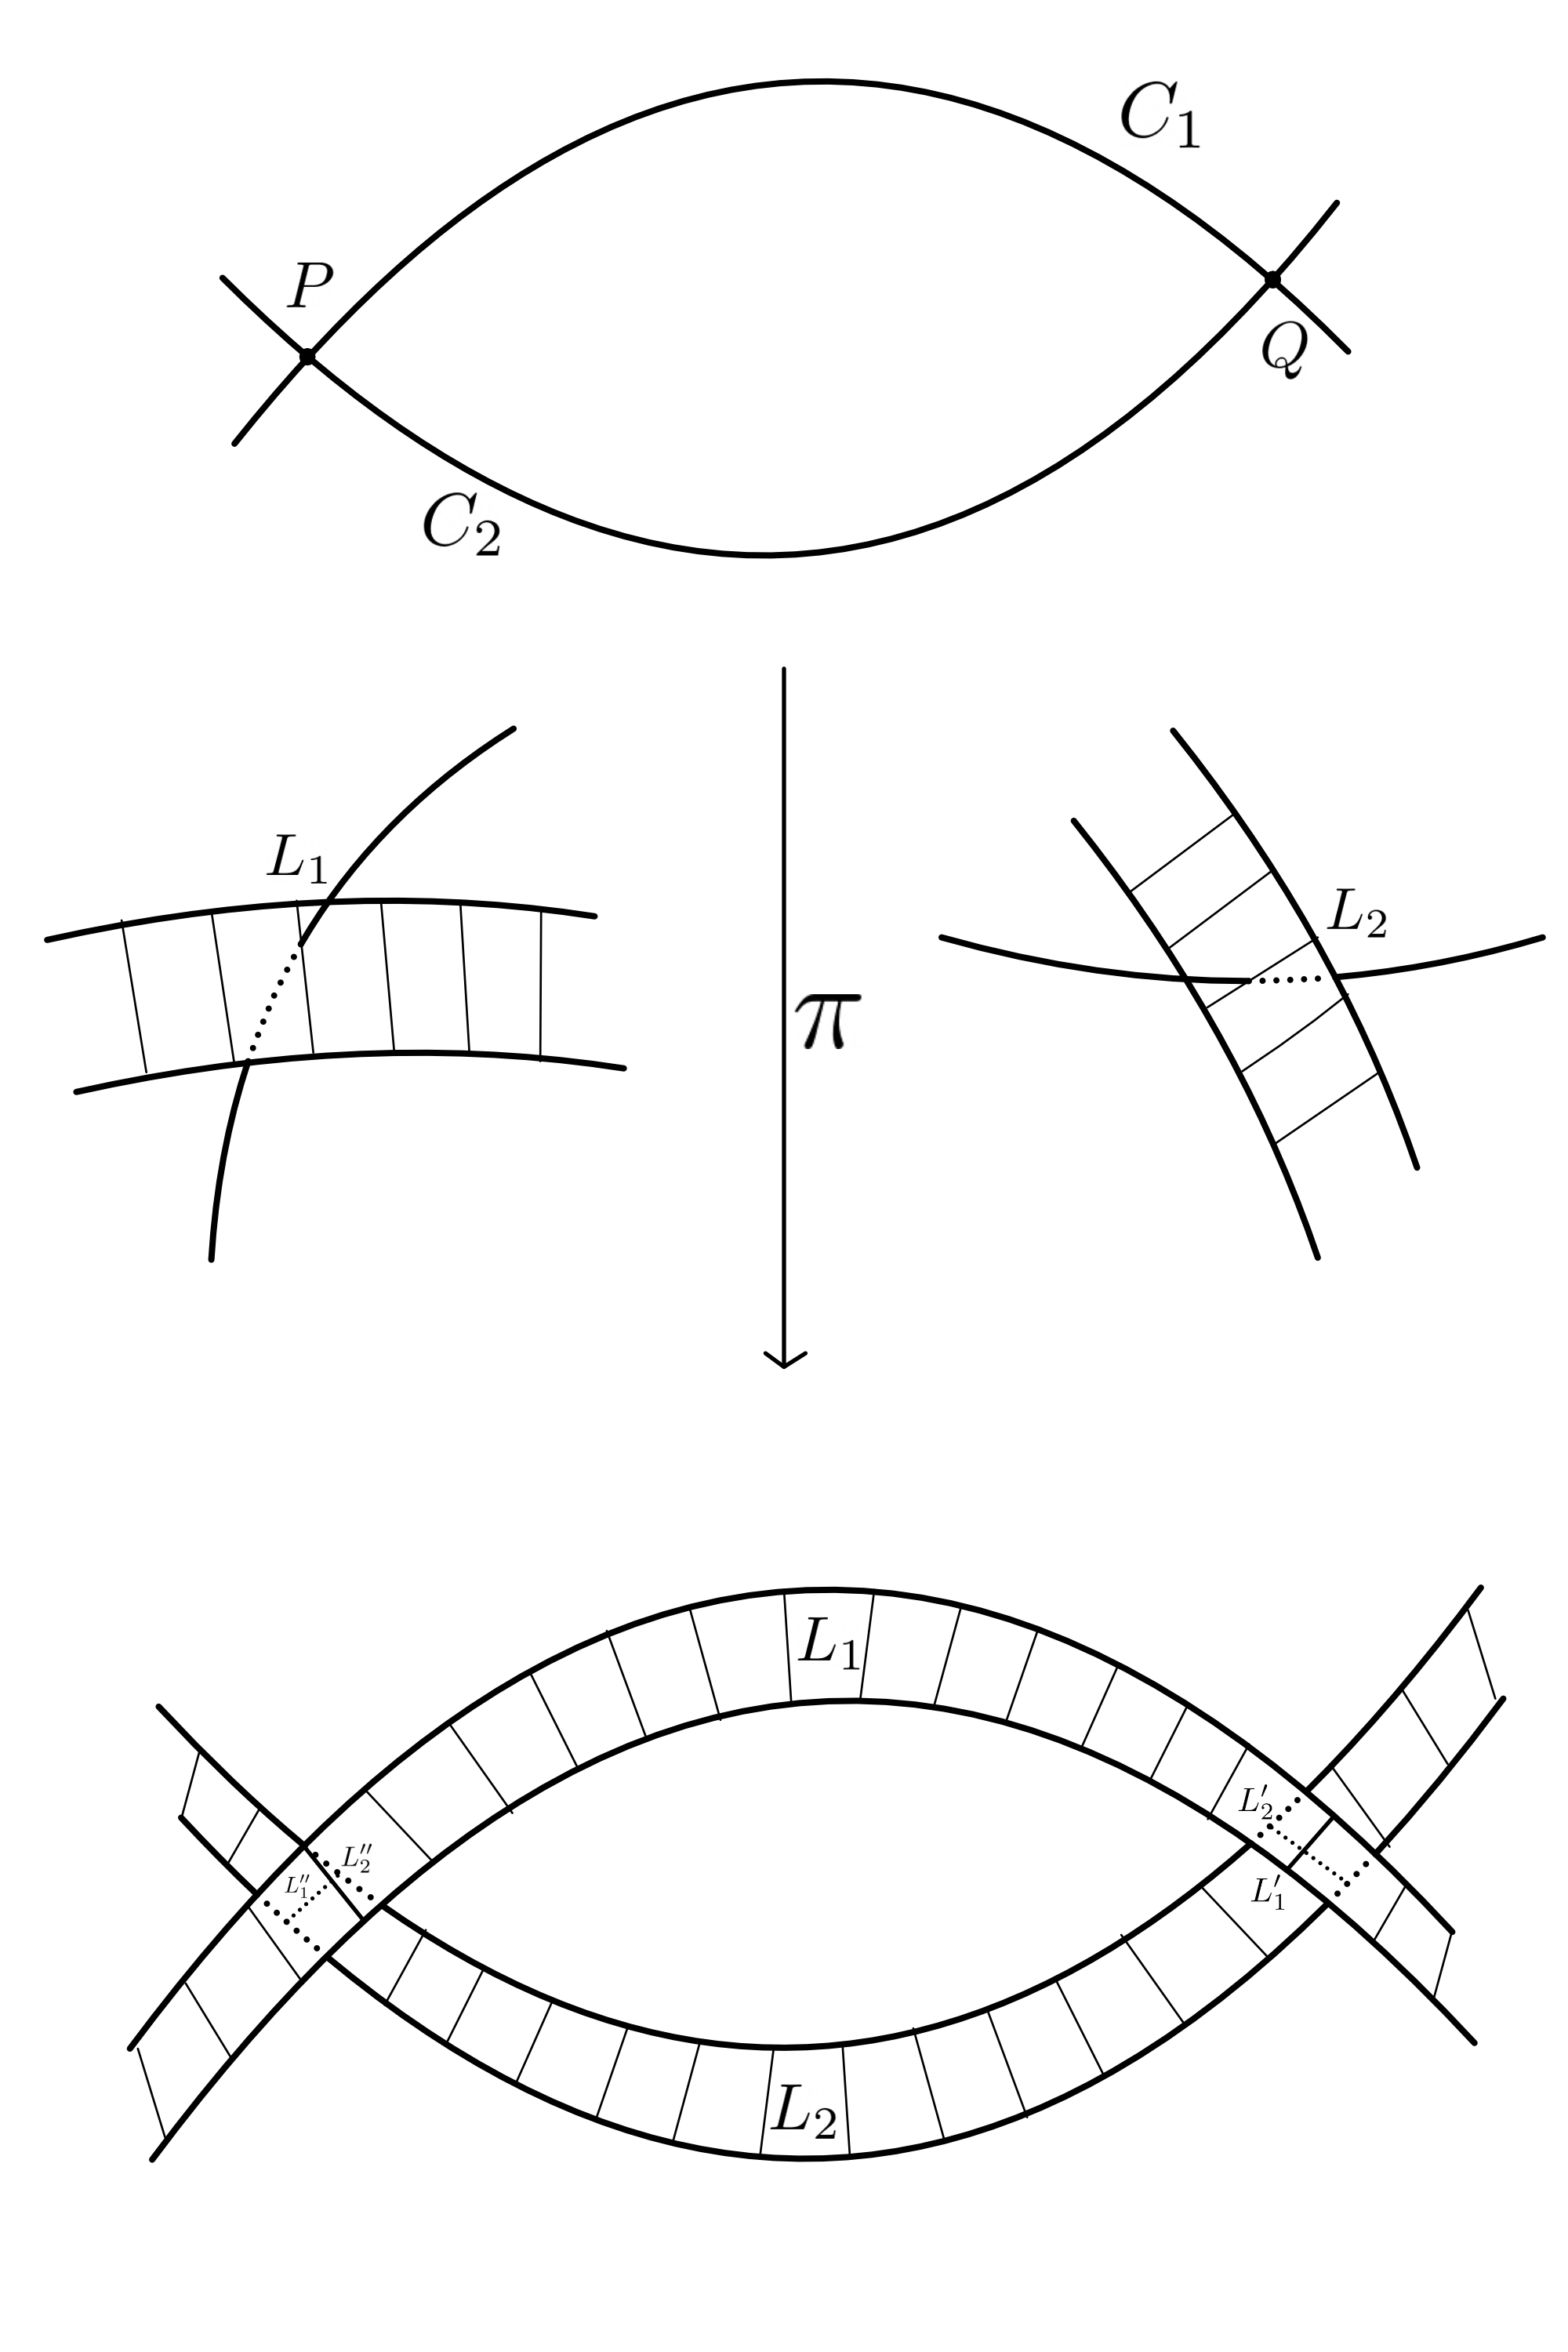
\includegraphics[width=0.4\linewidth]{Imagenes/Ejemplo Hironaka}
		\caption{Contraejemplo de Hironaka}
		\label{fig:ejemplo-hironaka}
	\end{figure}
\end{example}

\begin{remark}\parencite[Chap. VII, Sec. 6.4]{grauertremment}
	Continuando la observación \ref{espaciosdemoishezon}. El matemático americano \textit{Michael Artin} desarrolló unos objetos llamados \textbf{espacios algebraicos}. Intuitivamente, en lugar de utilizar esquemas afines como piezas locales de esquemas, los puntos en un espacio algebraico solo tienen vecindades étale y estas \enquote{piezas étale} luego deben pegarse. Los esquemas son naturalmente espacio algebraicos, pero una observación importante es que el contraejemplo de Hironaka genera un espacio algebraico que no es esquema. Además, se puede extender el funtor de analitificación al funtor
	\begin{equation*}
		(\_)^{an}:\{\text{espacios algebraicos de tipo finito }/\cc\}\longrightarrow\{\text{espacios complejos}\}.
	\end{equation*}
	En particular, Artin probó que este funtor induce la equivalencia categórica
	\begin{equation*}
		\{\text{espacios algebraicos propios de tipo finito}/\cc\}\cong\{\text{espacios de Moishezon}\}.
	\end{equation*}
	En otras palabras, todo espacio de Moishezon es de manera única un espacio algebraico, es decir, los espacios de Moishezon no se pueden pegar en general con la topología de Zariski como los esquemas, pero sí con la topología étale. Concluyendo que, para las necesidades de la geometría bimeromorfa, la categoría de esquemas suele ser insuficiente pues hay muy pocos objetos. Pero la categoría de espacios algebraicos sí lo es: no se puede abandonar esta categoría mediante modificaciones. 
\end{remark}

El resultado más importante de esta sección y conclusión final es el otro teorema demostrado por Moishezon.

\begin{theorem}[Teorema fundamental de Moishezon]\parencite{Moishezon1967}\label{fundamentaldemoishezon}
	Toda variedad de Moishezon y Kähler es algebrizable.
\end{theorem}

Este resultado conecta de forma conclusiva las distintas áreas de la geometría, pues significa que condiciones algebraicas y diferenciables en un contexto complejo imponen una estructura algebraica. De este modo, el teorema nos muestra la interacción entre la geometría diferencial, a través de la existencia de métricas de Kähler, y la geometría algebraica mediante la dimensión algebraica, dentro del marco de la geometría compleja, concluyen de manera natural al problema de algebrización abordado durante todo este trabajo. 
